\documentclass[
  	%draft,    % omit title page, listings, and particular chapters selected below using include only
	%german,   % titles for a thesis in German, A4 paper
	print,    % the printed version does not use colored links
	%final,    % removes all TODOs
]{tex/ttthesis}
\geometry{a4paper}

% Color Scheme http://colorschemedesigner.com/#3w40I--ALK-K-
% Base Color of the OVGU INF logo, tetraed, -45
\definecolor{blue1}{RGB}{0,105,180} % gray 95
\definecolor{blue2}{RGB}{40,87,121}
\definecolor{blue3}{RGB}{0,57,97}
\definecolor{blue4}{RGB}{76,166,230}
\definecolor{blue5}{RGB}{136,191,230}
\definecolor{orange1}{RGB}{255,144,0} % gray 133
\definecolor{orange2}{RGB}{171,121,56}
\definecolor{orange3}{RGB}{137,78,0}
\definecolor{orange4}{RGB}{255,181,84}
\definecolor{orange5}{RGB}{255,210,151}
\definecolor{green1}{RGB}{11,215,0} % gray 75
\definecolor{green2}{RGB}{52,144,48}
\definecolor{green3}{RGB}{6,116,0}
\definecolor{green4}{RGB}{88,241,80}
\definecolor{green5}{RGB}{148,241,143}
\definecolor{red1}{RGB}{253,0,6} % gray 86
\definecolor{red2}{RGB}{170,56,59}
\definecolor{red3}{RGB}{136,0,3}
\definecolor{red4}{RGB}{254,84,88}
\definecolor{red5}{RGB}{254,151,154}

\definecolor{background}{named}{white}
\definecolor{bgborder}{named}{black}
\definecolor{comment}{named}{red3}

\definecolor{blue}{named}{blue1}
\definecolor{green}{named}{green1}
\definecolor{red}{named}{red1}
\definecolor{orange}{named}{orange1}
 
\definecolor{pdflinkcolor}{named}{blue3}
\definecolor{pdfcitecolor}{named}{green3}

\usepackage{listings} % source code listings

%\renewcommand\lstlistingname{Quelltext}

\lstdefinestyle{java}{
%code formatting
	language=Java,
	tabsize=4,
	breaklines=false,
	basicstyle=\fontfamily{pcr}\footnotesize\selectfont,
	commentstyle=\fontshape{it}\color{darkgray}\selectfont,
	keywordstyle=\fontseries{b}\selectfont,
	stringstyle=\fontfamily{cmr}\selectfont,
%line numbering
	numbers=left,
	numberstyle=\footnotesize,
%frame properties
	captionpos=b,
	frame=single,%trblTRBL
	framesep=3pt,
	xleftmargin=4pt,
	xrightmargin=4pt,
	rulecolor=\color{bgborder},
}

\usepackage{pgfplots}
\usepackage{tikz}
	\usetikzlibrary{arrows,positioning,backgrounds,fit,trees} 
	\usetikzlibrary{fadings,shapes.geometric}
	\usetikzlibrary{decorations,scopes,calc,decorations.pathreplacing}

% Tortendiagramme
\newcommand{\slice}[4]{
  \pgfmathparse{0.5*#1+0.5*#2}
  \let\midangle\pgfmathresult

  % slice
  \draw[thick,
	%fill=background
	] (0,0) -- (#1:1) arc (#1:#2:1) -- cycle;

  % outer label
  \node[label=\midangle:#4] at (\midangle:1) {};

  % inner label
  \pgfmathparse{min((#2-#1-10)/110*(-0.3),0)}
  \let\temp\pgfmathresult
  \pgfmathparse{max(\temp,-0.5) + 0.8}
  \let\innerpos\pgfmathresult
  \node at (\midangle:\innerpos) {#3};
}
\newcommand{\mypiechart}[2]{
	\begin{tikzpicture}[scale=#1]
		\newcounter{a}
		\newcounter{b}
		\foreach \p/\t in {#2}
			{
				\setcounter{a}{\value{b}}
				\addtocounter{b}{\p}
				\slice{\thea/100*360}
							{\theb/100*360}
							{\p\%}{\t}
			}
	\end{tikzpicture}
}

% surrounding TODOs with this command, gives you the ability to remove all if necessary
\iffinal{
	\newcommand{\todo}[1]{}
	\newcommand{\todots}{}
}{
	\newcommand{\todo}[1]{{\color{comment}\textit{[#1]}}}
	\newcommand{\todots}{\todo{\ldots}}
}

% propositional formulas
\newcommand{\pand}{\wedge}
\newcommand{\por}{\vee}
\newcommand{\pnot}{\neg}
\newcommand{\pequals}{\Leftrightarrow}
\newcommand{\pimplies}{\Rightarrow}
\newcommand{\pnimplies}{\nRightarrow}
\newcommand{\patmostone}{\mbox{\textit{atmost1}}}
\newcommand{\pchooseone}{\mbox{\textit{choose1}}}

% mathematical definitions and theorems
\newtheorem{definition}{Definition}[chapter]
\newtheorem{theorem}{Theorem}[chapter]
\newtheorem{lemma}{Lemma}[chapter]

% print URLs not in Typewriter Font
\def\UrlFont{\rm}

% empty page without page number, continue on the next right page
\newcommand{\blankpage}{\clearpage{\pagestyle{empty}\cleardoublepage}}

% index stuff
\makeatletter
\def\mydotfill{\leavevmode\xleaders\hb@xt@ .44em{\hss.\hss}\hfill\kern\z@}
\makeatother
\def\bold#1{{\bfseries #1}}
\newbox\dbox \setbox\dbox=\hbox to .4em{\hss.\hss} % dot box for leaders
\newskip\rrskipb \rrskipb=.5em plus3em % ragged right space before break
\newskip\rrskipa \rrskipa=-.17em plus -3em minus.11em % ditto, after
\newskip\rlskipa \rlskipa=0pt plus3em % ragged left space after break
\newskip\rlskipb \rlskipb=.33em plus-3em minus.11em % ragged left before break
\newskip\lskip \lskip=3.3\wd\dbox plus1fil minus.3\wd\dbox % for leaders
\newskip \lskipa \lskipa=-2.67em plus -3em minus.11em %after leaders
\mathchardef\rlpen=1000 \mathchardef\leadpen=600
\def\rrspace{\nobreak\hskip\rrskipb\penalty0\hskip\rrskipa}
\def\rlspace{\penalty\rlpen\hskip\rlskipb\vadjust{}\nobreak\hskip\rlskipa}
\let\indexbreak\rlspace
\def\raggedurl{\penalty10000 \hskip.5em plus15em \penalty0 \hskip-.17em plus-15em minus.11em}
\def\raggeditems{\nobreak\hskip\rrskipb \penalty\leadpen \hskip\rrskipa %
\vadjust{}\nobreak\leaders\copy\dbox\hskip\lskip %
\kern3em \penalty\leadpen \hskip\lskipa %
\vadjust{}\nobreak\hskip\rlskipa}
\renewcommand*\see[2]{\rlspace\emph{\seename}~#1} % from makeidx.sty

\pgfplotsset{compat=1.7}

%*********************************************************************%
% META                                                                %
%*********************************************************************%
\ifgerman{
  \newcommand{\university}{Universität Passau}
  \newcommand{\school}{Fakultät für Informatik und Mathematik}
}{
  \newcommand{\university}{University of Passau}
  \newcommand{\school}{Department of Informatics and Mathematics}
}
\newcommand{\logo}{\includegraphics[height=3cm]{unilogo}}
\newcommand{\grouplogo}{
\includegraphics[height=1.5cm]{spl}}

\newcommand{\advisorone}{Dr.-Ing.\ Sven Apel}
\newcommand{\departmentone}{Software Product-Line Group}

\newcommand{\advisortwo}{Christian Kaltenecker, Ph.D.} 
\newcommand{\departmenttwo}{ Chair of Software Engineering I}

% Thesis kind
\ifgerman{\newcommand{\thesiskind}{Masterarbeit}}{\newcommand{\thesiskind}{Master's Thesis}}
%\ifgerman{\newcommand{\thesiskind}{Bachelorarbeit}}{\newcommand{\thesiskind}{Bachelor Thesis}}
%\newcommand{\thesiskind}{Diplomarbeit} %do not translate
%\ifgerman{\newcommand{\thesiskind}{Doktorarbeit}}{\newcommand{\thesiskind}{Dissertation}}

\newcommand{\theforename}{Rima Celita}
\newcommand{\thesurname}{Lewis}
\ifgerman{ 
	\newcommand{\thetitle}{Experimente zum Type-Checking von Softwareproduktlinien}
	\newcommand{\thedate}{31. März}
}{
	\newcommand{\thetitle}{Visualization of Performance-Influence Models}
	\newcommand{\thedate}{March 31}
	\newcommand{\thegermandate}{31. März}
}
\newcommand{\theyear}{2018}
\ifgerman{ 
	\newcommand{\thefullgermandate}{\thedate\ \theyear}
}{
	\newcommand{\thefullgermandate}{\thegermandate\ \theyear}
}


%*********************************************************************%
% SETUP                                                               %
%*********************************************************************%

% meta informations of the document
\hypersetup{
 pdfauthor={\theforename\ \thesurname},
 pdftitle={\thetitle}
}

% open index file
\ifnotdraft{\makeindex}

%*********************************************************************%
% THE DOCUMENT                                                        %
%*********************************************************************%

\begin{document}

% set the path where graphics are located
\graphicspath{{pics/}}

\ifnotdraft{
	\frontmatter
	\pagenumbering{roman}
	\newcommand{\theauthor}{\theforename\ \thesurname}
\newcommand{\theauthorr}{\thesurname,\ \theforename}
\begin{titlepage}
 \thispagestyle{empty}
 \begin{center}
  {\university}\\[0.4cm]
  {\school}\\[2.0cm]
  \begin{figure}[h]
   \hbox{}\hfill
    \begin{minipage}[t]{\textwidth}
      \begin{center}
        \logo
      \end{center}
    \end{minipage} 
   \hfill\hbox{}
  \end{figure}\ \\[0.4cm]
  {\large \thesiskind \\[1.6cm]}
  {\huge\bf \thetitle \\[1.6cm]}
  { \ifgerman{Autor:}{Author:}}\\[0.4cm]
  {\huge \theauthor}\\[0.8cm]
  {\large\thedate, \theyear}\\[0.8cm]
  {\ifgerman{Betreuer:}{Advisors:}}\\[0.4cm] 
  {\large
\advisorone
  }\\[0.2cm]
  {
\departmentone
  }\\[0.8cm]
  {\large
\advisortwo\ 
  }\\[0.2cm]
  {
\departmenttwo\ 
  }
%   \vfill
%   \begin{figure}[h]
%    \hbox{}\hfill
%     \begin{minipage}[t]{\textwidth}
%       \begin{center}
%         \grouplogo
%       \end{center}
%     \end{minipage} 
%    \hfill\hbox{}
%   \end{figure}
 \end{center}
\end{titlepage}

%%%%%%%%%%%%%%%%%%%%%%%%%%%%%%%%%%%%%%%%%%%%%%%%%%%%%%%%%%%%%%%%%%%%%%%%%%%%
%%% Titelrückseite: Bibliographische Angaben
%%%%%%%%%%%%%%%%%%%%%%%%%%%%%%%%%%%%%%%%%%%%%%%%%%%%%%%%%%%%%%%%%%%%%%%%%%%%

\thispagestyle{empty}
\vspace*{\fill}
\begin{minipage}{15.0cm}
\textbf{\theauthorr:}\\
\emph{\thetitle\\}
\thesiskind, \university, \theyear.
\end{minipage}
\newpage

	\ifgerman{\chapter*{Inhaltsangabe}}{\chapter*{Abstract}}

Configurable software systems have various configuration options such as encryption and compression. These configuration options and their interactions may have an influence on the non-functional properties of the system like performance or energy consumption. We use performance-influence models to interpret and understand the performance influences of certain configuration options or interactions on the non-functional properties of the system. However, the increasing complexity of performance-influence models for complex configurable software systems turns the interpretation into a difficult task. Therefore, as a solution to this issue, we present a tool to visualize the performance-influence models to make it easier to interpret them. For this thesis, we select 3 different visualization techniques. To demonstrate their usefulness, we validate these visualization techniques by performing an interview. In general, we find that one of the visualization technique outperformed the other in interpreting performance-influence models, but all the 3 visualization techniques certainly make interpreting performance-influence models easier
	\blankpage

	%\chapter*{Acknowledgements}
	%\ldots
	%\blankpage
}

%*********************************************************************%
% ACRONYMS                                                            %
%*********************************************************************%
  
% HOWTO: \gls{IDE} for singular or \glspl{IDE} for plural with 's
%\makeglossaries 
\newacronym{IDE}{IDE}{Integrated Development Environment} 
\glsaddall % use only if you have acronyms that occur only in graphics

%*********************************************************************%
% LISTINGS                                                            %
%*********************************************************************%
 
\ifnotdraft{
	{\parskip 0pt\tableofcontents} % toc bitte einzeilig
	\blankpage

	\ifgerman{
		\listoffigures
		\addcontentsline{toc}{chapter}{Abbildungsverzeichnis}

		\listoftables
		\addcontentsline{toc}{chapter}{Tabellenverzeichnis}

		\renewcommand{\lstlistlistingname}{Quelltextverzeichnis}
		\lstlistoflistings
		\addcontentsline{toc}{chapter}{Quelltextverzeichnis}

		\renewcommand*{\firstacronymfont}[1]{\emph{#1}}
		\printglossary[type=acronym,title=List of Acronyms,toctitle=Abkürzungsverzeichnis]
	}{
		\listoffigures
		\addcontentsline{toc}{chapter}{List of Figures}

		\listoftables
		\addcontentsline{toc}{chapter}{List of Tables}

		\renewcommand{\lstlistlistingname}{List of Code Listings}
		\lstlistoflistings
		\addcontentsline{toc}{chapter}{List of Code Listings}

		\renewcommand*{\firstacronymfont}[1]{\emph{#1}}
		\printglossary[type=acronym,title=List of Acronyms,toctitle=List of Acronyms]
	}
}

%*********************************************************************%
% CHAPTERS                                                            %
%*********************************************************************%

\mainmatter
\pagenumbering{arabic}

\ifgerman{\chapter{Einführung}}{\chapter{Introduction}}
%- Hintergrund
%- Motivation
%- Ziele
%- Aufgaben
%- Allgemeine Beschreibung des Projektes
%- Worum geht es in dieser Arbeit?
%- Wer hat die Arbeit veranlasst und wozu?
%- Wer soll von den Ergebnissen profitieren?
%- Welches Problem soll gelöst werden? Warum?
%- Unter welchen Umständen braucht man eine Verbesserung?
%- Was ist der Stand der Technik?
%- Welche noch offenen Probleme gibt es?
%- Worin unterscheidet sich mein Ansatz von den bisherigen?
%- Welche Ziele hat die Arbeit?
%- Wie will ich diese Ziele erreichen?
%- Was habe ich im Einzelnen vor? 


\section{Goal of this Thesis}
Performance-Influence Models helps to understand how performance of a software system is affected, but when a performance-influence model is very large, it is not easily readable. The complexity of the model can increase when the configuration features of a software system increases.
The model in its original format is not easy to draw conclusions.
As a solution to this problem, we use these models to map into several visualizations, based on which the user/developer can draw conclusions easily.
The motivation behind the thesis is to understand large performance-influence models easily. which cannot be done in its original text format.
Visualization of any data makes it easier to understand it, for example to know the outlier in a large set of data.

Most of the software systems are configurable to the user. The  software systems when configured affects certain functional and non-functional requirements of the software. In this thesis we focus on non-functional requirements, for example Performance. These software systems should be optimized in a way to affect performance positively.


\ifgerman{\chapter{Grundlagen}}{\chapter{Background}}
\label{background}

%- Allgemeine Wissensgrundlagen des Fachgebiets
%- Spezielle Grundlagen, die für das Verständnis erforderlich sind
%- Rahmenbedingungen für die Arbeit
%- Ausführungen zum Stand des Wissens / der Technik
%Als Leitprinzip gilt: Nur Informationen erwähnen, die
%- später benötigt werden,
%- notwendig sind, um die Arbeit oder ihre Motivation zu verstehen
%Das heißt insbesondere,
%- keine Inhalte aus Lehrbüchern, außer
%- diese werden benötigt, um Problemstellung oder Lösungsweg zu definieren.

% \gls{IDE}
 
A software or a system with different configuration options is called configurable software system. A configuration option add a definite functionality to the system, it can be optional or mandatory. A configuration option can be selected or deselected. An example for Configuration option can be compression and encryption.
when several configuration options are selected at the same time, they may interact with each other, when they do it is called an Interaction.
Often times, a user or a developer is interested in knowing how the configuration options and/or interactions have an impact over the performance of the system. To know the performance influence we use a tool called 'SPL Conqueror'.
SPL Conqueror takes as an input a Configurable software system, and produces a set of valid Performance-Influence models as an output.

An example for Performance-Influence Model: 

\begin{equation*}
  \pi {(c)} = \overbrace{\underbrace {3}_{Coeff.} \cdot  \underbrace{{C(A)}}_{Option}}^{Term 1}  + \overbrace{ \underbrace{5}_{Coeff.} \cdot \underbrace{{C(B)}}_{Option}}^{Term 2} + \overbrace{\underbrace{0}_{Coeff.} \cdot \underbrace{{C(C)}}_{Option}}^{Term 3} - \overbrace{\underbrace{4}_{Coeff.} \cdot \underbrace{{ C(A)} \cdot {C(B)}}_{Interaction}}^{Term 4}
\end{equation*}


Every performance-influence model consists of a set of terms. Each term has the participating configuration option/interactions and a co-efficient. This co-efficient indicates the performance that the configuration option/interaction contributes towards the total performance of the system.
Performance here is calculated in terms of its execution time. A positive value indicates that the performance of the system decreases, whereas a negative term indicates that it increases the performance of the system.
These Performance-Influence models can be visualized, which makes it easier to interpret them. Once we have the visualization we can identify the most relevant configuration option/interaction.
A software may have an upgraded version, in this case we can compare the current and the upgraded versions of the software to identify the differences in the performance influence the configuration options/interactions may have.
As and when the software is upgraded to add new configuration options, the size of the visualization increases to reflect the newly added configuration options. The visualization scales as the software keeps adding or removing configuration options.
                                                                       

 
 
\todots{

  - Explain what is 
	                -> configurable software systems
	                -> Performance-Influence Models
	                -> Configuration options
	                -> Interactions
	                -> Positive and negative influences
	            - Research Questions
	            Research Questions :
General : can we use the visualization techniques to visualize Performance-Influence models?
 1. Can we use the visualization techniques to identify relevant properties of one performance-influence models?
 2. Can we use the visualization techniques to compare two performance-influence models?
 3. How do visualization techniques scale?
	            - Visualization techniques 
	            - Things explained in the warm-up phase of the interview
	            - No need to explain Feature Models
	            - Use one example of Preformance-Influence Model throughout the documentation
	            - Example should include configuration options, Interactions, positive terms, negative terms-}
\chapter{Methodology}
\label{example}
%In diesem Kapitel beschreiben Sie Ihren eigenen Beitrag
%- Es muss klar sein, worin die eigentliche Innovation besteht#

\section{Research Questions}
For this thesis we have selected 3 research questions. The first question : Can we use the visualization techniques to identify relevant properties of one performance-Influence model? The performance-influence models are of the format mentioned below:

\begin{equation*}
  \pi {(c)} = \overbrace{\underbrace {3}_{Coeff.} \cdot  \underbrace{{c(A)}}_{Option}}^{Term 1}  + \overbrace{ \underbrace{5}_{Coeff.} \cdot \underbrace{{c(B)}}_{Option}}^{Term 2} + \overbrace{\underbrace{0}_{Coeff.} \cdot \underbrace{{c(C)}}_{Option}}^{Term 3} - \overbrace{\underbrace{4}_{Coeff.} \cdot \underbrace{{ c(A)} \cdot {c(B)}}_{Interaction}}^{Term 4}
\end{equation*}

The set of valid performance-influence models are put into a csv file. And these csv files are used as an input for the visualization. 

From the visualizations we can identify the data point that is either the highest or lowest point that influences the systems performance the most.

Second research question : Can we use the visualization to compare two performance-influence models?. Many times a version of a software needs to be compared to its next version to check how the two versions differ in terms of its performance. In this case, we have two performance-influence models in one csv file, and use this as an input to the visualization. hence comparison of two different performance-influence models can be done, and identify if the same configuration option causes a spike in performance in either of the versions.

Third research question : How do the visualizations scale?. when a configurable software has added new configuration options, new performance-influence models are derived to reflect its performance influence over the system. The new performance-influence models are then used as an input to the visualization. Scaling can be of two types. One, addition of new configuration option. Two, addition of new performance-influence model to the same csv file. Both of the types of scaling are implemented in the thesis.

\section{Why the above Research Questions?}
The research questions are selected based on number of performance-influence models we visualize at the same time. When we have only one performance-influence model, we would like to know the configuration option that has affected the performance the highest, it can be maximum performance increase or decrease. 

when we look at the two performance-influence models, we are basically comparing the two and finding out the configuration that either differs the most or is the most similar. The configuration option that differs the most can indicate that this configuration option has caused a performance spike in one of the versions, it can be positive or negative spike. The configuration option that have been the most similar indicate that in the second version of the software, this configuration option remained unaffected.

when we look at more than 2 performance-influence models, we have comparing several versions of the same software with increasing configuration options in each versions. This visualization helps to see what would be the outliers, or which set of performance-influence models have share similar set of influences.

\section{How do we plan on getting the answers to these questions?}

we use three different visualization tecnhiques to help us answers the research questions. Each visualization has its own steps to get to the answers.

Question 1: The  most relevant configuration option or interaction would be the one which makes highest positive or most negative effect. The configuration option or interaction which makes zero effect would be also of interest here.

 Radar Chart:  For this visualization, we identify the data point that is plotted far most in the outer circle which indicates that it makes the most negative effect on performance, or the data point that is plotted closer most to the inner circle which indicates that it makes the most postive effect on performance. If there are two data points that are very close to each other, we can use the tooltip to see the exact value that it contributes. Hence we can come to a conclusion on one single data point that would make the most postive or the most negative effect on performance of the entire system. For the configuration option or interaction which makes zero effect, we need to identify the data point which is plotted with a white round symbol.

 Text Plot : For this visualization, we identify the data point that is closest to either of the border lines of the plot. The data point which is closest to the left border line indicates that it makes the most positive effect on the performance. whereas the data point which is closest to the right border line indicates that it makes the most negative effect on the performance. If there are two data points which are very close to each other and are not able to be distinguished, we can use the tooltip to hover over both the data points to look at the exact value that it contributes and hence know the most relevant configuration option or interaction. For the configuration option or interaction that makes zero contriubution towards the performance, we need to identify the data points marked with an inner white marker symbol. These are the configuration options or interactions which makes no contribution towards the performance of the entire system.

 Ratio Plot : For this visualization, we know that the bars are sorted according to the amount of performance it contributes. Hence it is very easy to identify the configuration option or interaction which makes the highest performance affect. It the first bar in the visualization, and the bar which is to the extreme right indicates that it makes the lowest performance affect. But, this conclusion is when we do not consider the sign of the data points. For example, the first bar makes the highest performance affect, but we do not know if it makes most positive or most negative effect on performance, it can be either postive or negative. For that configuration option or interaction that makes zero effect on performance, it is again hard to identify since these configuration options are not plotted in the graph at all.

 Question 2 : Often times a developer or an user would need to compare two versions of the same software to identify if there are any performance spikes or an introduction of a performance bug. In this case, we use the performance-influence models of the two different versions in the same csv files as different groups. The different groups are plotted as two different plots in the same graphs hence the comparision is easier.

we can use the two different plots to identify the configuration option or interaction that are the most similiar to each other, which indicates that the performance contributed by this configuration option or interaction is not affect in the newer version. we can also use the different plot to identify the configuration option or interaction which are most different to each other, which indicates that the performance contributed by this configuration option or interation is affected the most by introduction of the newer version. This can also indicate the introduction of the performance bug.

 Radar Chart: For this visualization, we need to identify the corresponding data point in both the plots which are most closer to each other or most far away from each other. The data points which are most close to each other indicate that  corresponding configuration option or interaction contributes the same/ similar amount of performance to the performance of the entire system. The data points which are most far away from each other indicate  that the corresponding configuration option or interaction has a spike in performance in the newer or older version of the software. It can also indicate that the newer version of the software has introduced a performance bug with respect to the corresponding configuration option or interaction. 


 Text Plot : For this visualization, we need to identify the corresponding data point in both the plots which are most closer to each or the most far away from each other. Both of which make the same conclusion as mentioned above in the radar plot.

 Ratio Plot: For this visualization, we need to identify the bars (configuration option or interaction) which are most similar or same in size and color, which indicates the configuration option or interaction that makes same or similar amount of performance in the newer version of the software as that of the older version. we can also identify the bar that would has the highest difference in the size of the bars but are of the same color. This configuration option or interaction indicates that it contributes to a lot of performance in the newer version than that of the older version. This contribution can be a performance increase or decrease, if its performance increase in the newer version it can also indicate that this configuration option or interaction has introduced a performance bug in the newer version of the software.

 Question 3: Scaling of the visualization techniques can be in two different ways. one, addition of new configuration options or interactions. second, addition of new groups/ plots to the same graph.

Radar Plot and Text Plot: 
Addtion of new configuration option /interaction: Adding new features to configurable softwares indicates that a new configuration option and or an interaction is added to the newly produced performance-influence model. As and when the performance-influence model increases, the size of the visualization also increases in the same order.
Addition of new gorups to the same graph: For comparision of several versions of the software, several groups/ performance-influence models of individual versions are put in the same csv file. Each individual version is mapped as a different plot in the same visualization, which makes comparision of all the versions easier.

Ratio Plot : 
Addtion of new configuration option /interaction: Addition of new configuration option or interaction is added as a new bar in the visualization. As and when the size of the performance-influence model increases, the size of the visualization increases in terms of the number of bars the visualization consists. 
Addition of new gorups to the same graph: For comparision of several versions of the software, several performance-influence models are put in the same csv file and this file is used as an input to the visualization. Each individual version is mapped as a different plot/set of bars in the same visualization, making comparision of several versions at the same time easier.

\section{Interview}

To test the tool and get some feedback, we interviewed possible users of the tool to use it and answer several questions based on the visualization of performance-influence models. The interview consisted of an initial warm--up phase, where the interviwee is given a brief explaination of performance-influence models, configurable software systems, configuration option, interaction etc. The interviewer also explains in brief the working of the tool, so that the interviwee can use the tool themselves to answer the questions.
The questions are separated based on the number of performance-influence models the questions they include. There are three sections, one performance-influence model, two performance-influence models and many performance-influence models. Each section has several questions, each question includes a different performance-influence model for each of the visualization type, namely radar plot, text plot and ratio plot. 
The questions themselves are answered on likert scale indicating how easy or difficult it is for a user to derive the answer the question. If the questions have a definite answer, an area to fill in the answer is provided for the user to enter the answer. Also each question has a comments or feedback area to fill in, if the user has feedback or some input for possible betterment of the visualizations.
Each question is in form of a link, which when clicked opens a new visualization for the user to answer the question.

\section{Questionnaire}
The questionnaire is divided into three sections. Each section having set of questions belonging to either simple performance-influence model or complex performance-influence model.

One performance-influence model
  Question 1: Which is the most relevant configuration option or interaction?
  Question 2: Which is the configuration option or interaction that leads to highest performance increase or decrease?

Two performance-influence models
 Question 1: Which is the configuration option or interaction where the performance-influence models differs the most?
 Question 2: Which is the configuration option or interaction where the performance-influence models are the most similar?

Many performance-influence models
 Question 1: which pair of performance-influence models share a large set of influences?

 Each question has 3 sub sections for three different types of visualizations.

\section{Acronyms}

This template makes advantage of the glossaries package to support acronyms. The first occurence of an acronym is replaced by its definition (e.g., \gls{IDE}). All other occurences are replaced by the acronym (\gls{IDE}). The glossaries package also supports plural---\glspl{IDE}.

\glsreset{IDE}
Sometimes you want to make sure, that the long version is used, even if \gls{IDE} was inserted before.
 
\section{Citation}

There are several types of literature. The most citations are workshop and conference papers. Please use the inproceedings-tag for those citations (e.g., \cite{KAK:GPCE09}). You should have short-hands for workshop and conference names to be sure the naming is consistent and uniform (see our BibTeX files how to do that).
 
Slightly different are articles published in journals (e.g., \cite{KG:SME06}). Make sure you that the volume and number-tags are present and that no inproceeding is tagged as article or vice versa.

You might want to take a look at the example BibTeX file to find out how to cite books~\cite{CE:BOOK00}, technical reports~\cite{KCHNP:TR90}, websites~\cite{Coq:website}, PhD theses, or master theses~\cite{B:PHD03,R:MT09}.

\section{Formulas}
 
There are different types of mathematical environments to set formulas. The equation $E=m\cdot c^2$ is an inline formula. But you can also have formulas at a separate line (see \vref{eq:ex}).

	\begin{equation}\label{eq:ex}
			P=\bigl(\mathcal{A}\pimplies(\mathcal{B}\pequals\mathcal{C})\pand(\mathcal{B}\pequals\mathcal{D})\bigr)\pand(\mathcal{B}\pimplies\mathcal{A})\pand(\mathcal{C}\pimplies\mathcal{A})\pand(\mathcal{D}\pimplies\mathcal{A})
	\end{equation}

If you need multiple lines that are aligned to each other, you might want to use the following code.

	\newcommand{\fG}{\mbox{GraphLibrary}}
	\newcommand{\fE}{\mbox{Edges}}
	\newcommand{\fA}{\mbox{Algorithms}}
	\newcommand{\fD}{\mbox{Directed}}
	\newcommand{\fU}{\mbox{Undirected}}
	\newcommand{\fN}{\mbox{Number}}
	\newcommand{\fC}{\mbox{Cycle}}
	\begin{eqnarray*}
	&& \fG\\
	&\pand& (\fG \pimplies \fE) \pand (\fE \por \fA \pimplies \fG)\\
	&\pand& (\fE \pequals \fD \por \fU) \pand (\pnot \fD \por \pnot \fU)\\
	&\pand& (\fA \pequals \fN \por \fC)\\
	&\pand& (\fC \pimplies \fD).\\
	\end{eqnarray*}

\section{Graphics}

In \vref{fig:ex}, we give a small example how to insert and reference a figure.

\begin{figure}[htbp]
	\centering
		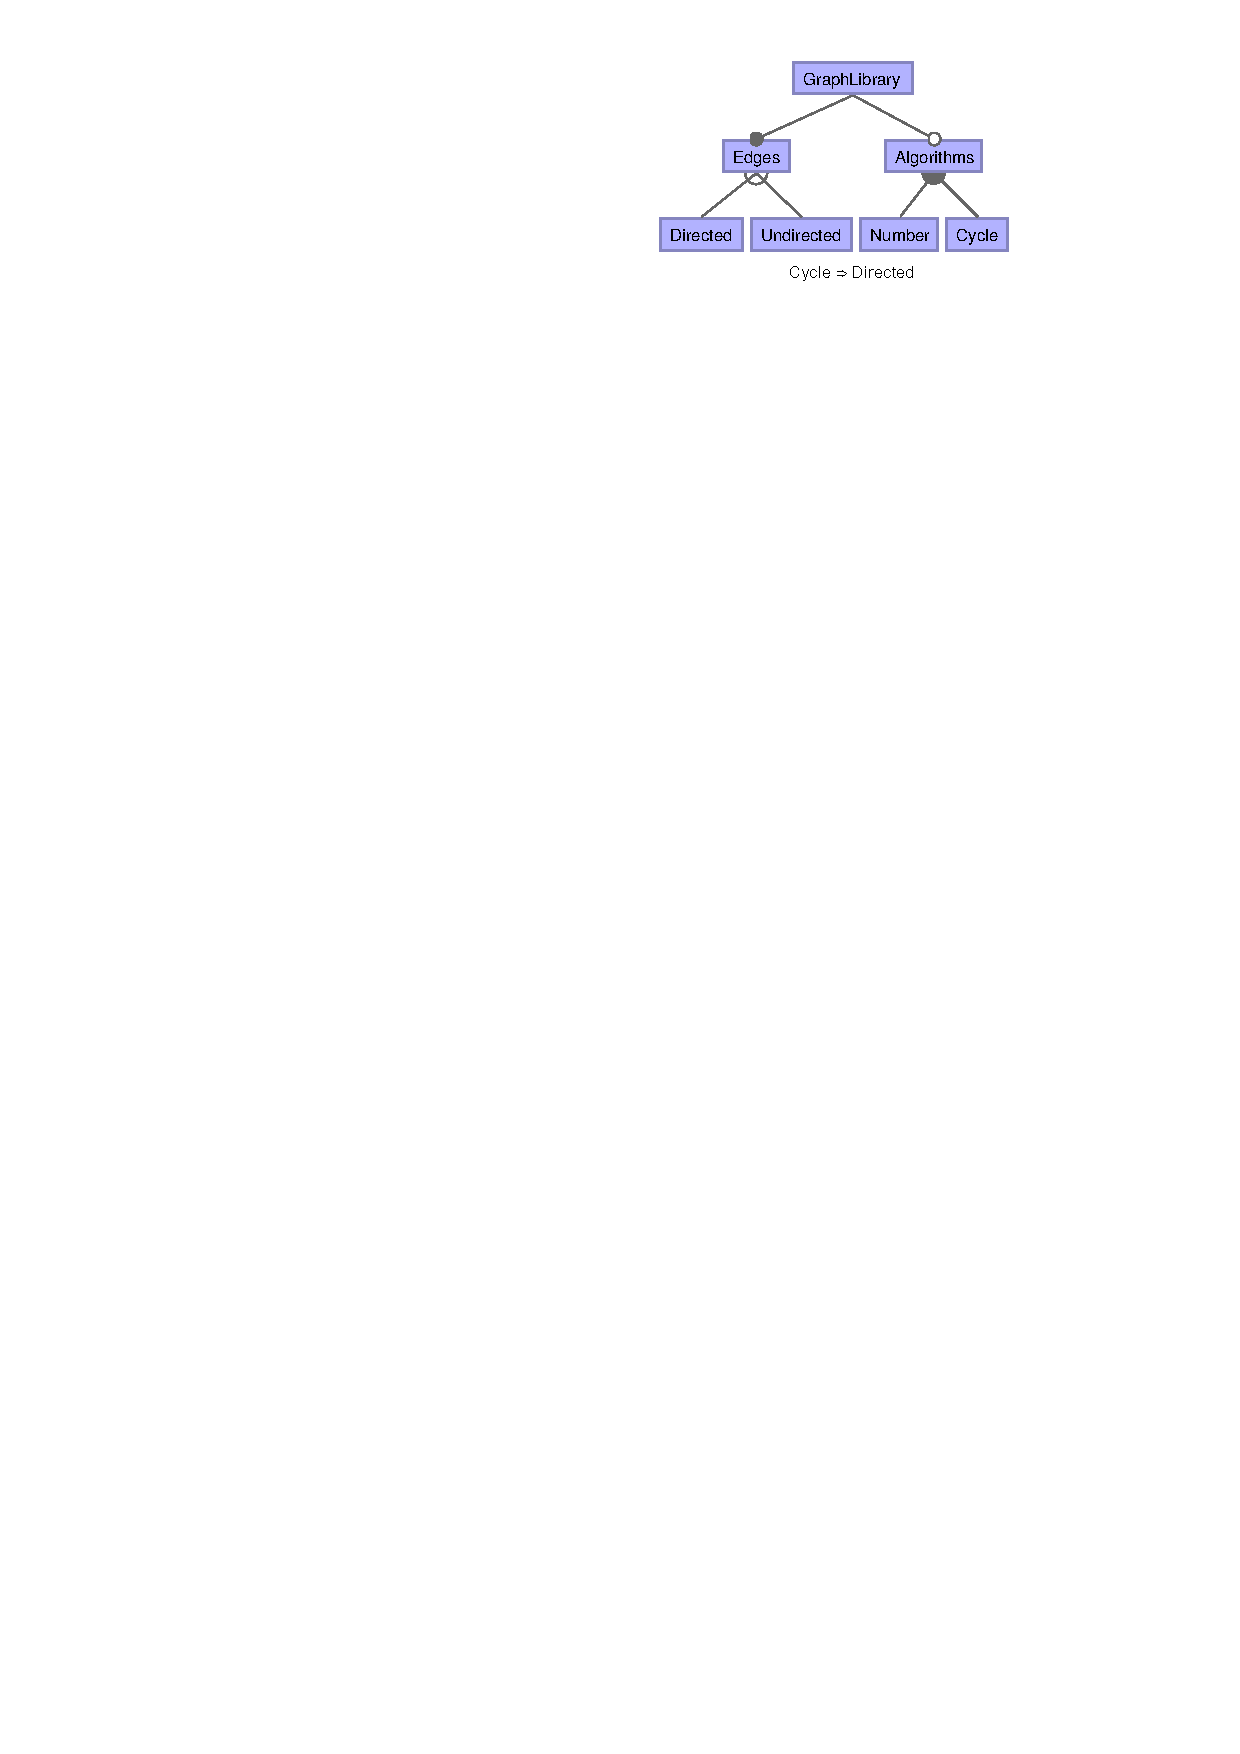
\includegraphics[scale=1.25]{example}
	\caption{A feature model representing a graph product line}
	\label{fig:ex}
\end{figure}

\section{Tables}

\vref{tab:ex} shows the result of a simple tabular environment.

\begin{table}[htbp]
	\centering
		\begin{tabular}{cc}\toprule
			Group Type & Propositional Formula\\\midrule
			And & $(P \pimplies C_{k_1} \wedge\ldots\wedge C_{k_m}) \pand (C_1\vee\ldots\vee C_n \pimplies P)$\\\addlinespace
			Or & $P \pequals C_1\vee\ldots\vee C_n$\\\addlinespace
			Alternative & $(P \pequals C_1\vee\ldots\vee C_n) \pand \mbox{atmost}1(C_1,\ldots,C_n)$\\
			\bottomrule
		\end{tabular}
	\caption{Mapping a feature model to a propositional formula}
	\label{tab:ex}
\end{table}

\section{Code Listings}

In \vref{lst:ex}, we give an example of a source code listing. 

\begin{lstlisting}[style=Java,float=htb,caption={Java source code},label={lst:ex}]
class A extends Object {
	A() { super(); }
}
class B extends Object {
	B() { super(); }
}
class Pair extends Object {
	Object fst;
	Object snd;
	Pair(Object fst, Object snd) {
		super(); this.fst=fst; this.snd=snd;
	}
	Pair setfst(Object newfst) {
		return new Pair(newfst, this.snd);
	}
}
\end{lstlisting}

\chapter{Experiment Setup}
%In diesem Kapitel beschreiben Sie,
%- wie Sie versucht haben, Ihre Arbeit (z.B. Programm, Theorie, oder Algorithmus) zu verifizieren
%- Hierfür haben Sie bereits im Kapitel 3 Prognosen oder Qualitätskriterien aufgestellt, die Sie hier überprüfen
%Zu jeder zu überprüfenden Eigenschaft sollten Sie
%- ein geeignetes Experiment entwerfen, um diese Eigenschaft zu überprüfen
%- dieses Experiment beschreiben und durchführen
%- die Ergebnisse geeignet präsentieren und kommentieren

%wie lange dauert das schlussfolgern bei bestimmten veränderungen?
%wie lange für komplett unterschiedliche?



\chapter{Evaluation}
\label{evaluation}

In this chapter, we present and discuss the results of the interview. We evaluate the research questions from the results obtained from the interview. We assess the results by using the correctness of the answers, the time needed and the difficulty rating giving by the interviewees. Correctness is presented in \hyperref[sec:4.1]{Section 4.1} and time measurements is presented in \hyperref[sec:4.2]{Section 4.2}. We also present the results of difficulty rating in \hyperref[sec:4.3]{Section 4.3}. We answer our research question from the presented results in \hyperref[sec:4.4]{Section 4.4}. In \hyperref[sec:4.5]{Section 4.5}, we discuss our findings with respect to the results. We also present certain factors in \hyperref[sec:4.6]{Section 4.6}, that might have influenced our interview unfavorably. Finally, in \hyperref[sec:4.7]{Section 4.7}, we present feedback given by the interviewees on how the visualization of performance-influence model tool can be improved. 

\section{Correctness}
\label{sec:4.1}
We check the answers given by the interviewees to the questions asked in the questionnaire. We evaluate how often an interviewee answered the question correctly. The evaluation is done with respect to each question and each use case; simple and complex. \hyperref[table:correctness]{Table 4.1} presents the relative number of correct answers given for each use case with its summary per question. 
 
\begin{table}[!htbp]
\centering
\small
\begin{tabular}{lccccccc}
\toprule   
 Input & Use Case & Radar Plot  & Text Plot  & Ratio Plot \\ 
\midrule
& Simple & 100\% &  100\% & 88.8\%\\ 
Q1  & Complex &  100\% &  100\% &  77.7\%\\ 
\midrule
& Summary &  100\% &  100\% &  83.83\%\\
\bottomrule
& Simple & 70\% &  100\% & 60\%\\ 
Q2 & Complex & 100\% & 100\% & NA\\ 
\midrule
& Summary & 83.34\% & 100\% &  60\%\\
\bottomrule
& Simple & 100\% &  100\% & 100\%\\ 
Q3 & Complex & 22.23\% & 100\% & 66.66\%\\ 
\midrule
& Summary & 61.11\% & 100\% &  66.66\%\\
\bottomrule
& Simple & 100\% &  88.89\% & 22.23\%\\ 
Q4 & Complex & 88.89\% & 88.89\% & 55.55\%\\ 
\midrule
& Summary & 94.45\% & 88.89\% &  26.66\%\\
\bottomrule
& Simple &  88.89\% &  88.89\% & 33.34\%\\ 
Q5 & Complex & 33.34\% & 100\% &  88.89\%\\ 
\midrule
& Summary & 77.77\% & 94.44\% &  61.11\%\\
\bottomrule
& Simple &  33.34\% &  22.22\% & 88.88\%\\ 
Q6 & Complex & 55.55\% & 77.77\% &  77.77\%\\ 
\midrule
& Summary & 61.11\% & 50\% & 83.33\%\\
\bottomrule
\end{tabular}
\label{table:correctness}
\caption[Correctness Table]{The relative number of correctly answered questions in the interview for the different visualization techniques
across the different questions and complexities.} 
\end{table}
 
\section{Time Measurements}
\label{sec:4.2}
The second factor to evaluate the research questions, is by taking time measurements.

\begin{table}[!htbp]
\centering
\begin{adjustbox}{width=1\textwidth}
\begin{tabular}{@{\extracolsep{4pt}}lccccccc}
\toprule   
   &  Radar Plot  & Text Plot  & Ratio Plot  & Radar Plot  & Text Plot  & Ratio Plot \\ 
Input & <  & <  & < & > & > & > \\
   &  Text Plot & Ratio Plot & Radar Plot & Text Plot & Ratio Plot & Radar Plot\\
\midrule
Q1 Simple  & 0.535 & 0.638 & 0.5 & 0.5 & 0.395 & 0.535\\ 
Q1 Complex & 0.535 & 0.464 & 0.604 & 0.5 & 0.570 & 0.429\\ 
Q2 Simple  &  0.855 & \textbf{0.010} & 0.953 & 0.165 & 0.991 & \textbf{0.055}\\ 
Q2 Complex & 0.811 & \textbf{--} & \textbf{--} & 0.213 & \textbf{--} & \textbf{--}\\ 
Q3 Simple  & 0.5 & \textbf{0.004} & 0.994 & 0.535 & 0.996 & \textbf{0.006}\\ 
Q3 Complex & 0.982  & \textbf{0.004} & 0.701 & \textbf{0.021} & 0.996 & 0.329\\ 
Q4 Simple & 0.395 & \textbf{0.001} &  0.999 & 0.638 & 0.998 & \textbf{0.000}\\ 
Q4 Complex & 0.638 & \textbf{0.006} & 0.996 & 0.395 & 0.994 &  \textbf{0.004}\\ 
Q5 Simple  & 0.973 & 0.055 & 0.701 & \textbf{0.031} & 0.953 & 0.329\\ 
Q5 Complex & 0.429 & 0.125 & 0.670 & 0.604 & 0.891 & 0.361\\ 
Q6 Simple  & 0.464 & 0.760 & 0.329 & 0.570 & 0.268 & 0.701\\ 
Q6 Complex & 0.535 & 0.188 &  0.811 & 0.5 & 0.834 & 0.213 \\ 
 \midrule
Q1 Simple \& Complex & 0.581 & 0.493 &  0.544 & 0.430 & 0.581 & 0.468\\ 
Q2 Simple \& Complex & 0.920 & \textbf{0.004} &  0.973 & 0.084 & 0.995 &  \textbf{0.030}\\ 
Q3 Simple \& Complex & 0.894 & \textbf{0.000} & 0.976 & 0.111 & 0.999 & \textbf{0.025}\\
Q4 Simple \& Complex & 0.518 & \textbf{0.000} &  0.999 & 0.493 & 0.999 & \textbf{0.000} \\
Q5 Simple \& Complex & 0.899 & \textbf{0.028} & 0.559 & 0.105 & 0.973 &  0.454\\
Q6 Simple \& Complex & 0.455 & 0.369 & 0.665 & 0.556 & 0.642 & 0.346\\
\bottomrule
\end{tabular}
\end{adjustbox}
\label{table:time}
\caption[Mann-Whitney U Test]{Mann-Whitney U test results for the different visualization techniques across the different questions and complexities.} 
\end{table}

Time is measured on how long an interviewee took to answer a question. This is done to compare if an interviewee took a long time to answer a complex use case than a simpler one or to check if one of the visualization techniques was more time consuming than others.

We will conduct the \textit{Mann–Whitney U test} in this section.

\subsection{Mann–Whitney U test}
We use the Mann-Whitney U test to determine if one sample is significantly better than another sample when time is considered as a factor. A sample is significantly better than another if the p value of the test is less than 0.05. \hyperref[table:time]{Table 4.2}, presents the results for Mann–Whitney U test. The significant values are marked in bold.

In our case, we determine if one group of time measurement is significantly better than another group of time measurement. We compare time measurement groups between the radar plot, the text plot, and the ratio plot. 

Here we try to find, if a visualization technique consumed significantly less time than other visualization techniques. For instance, radar plot $<$ text plot implies if the radar plot is better than the text plot if the Mann–Whitney U test value is less 0.05. Similarly, radar plot $>$ text plot implies if the radar plot is worse than the text plot. 

\section{Difficulty Rating}
\label{sec:4.3}

The difficulty rating in our thesis is assessed using Likert scales. This scale helps us determine the difficulty perception of the interviewee based on the visualization technique and the complexity of the performance-influence model.

The difficulty rating is considered as a factor for the evaluation of research questions. The interviewee selects the difficulty rating on how easy or difficult it was to answer a question. This rating corresponds to the time taken by the interviewee to answer the question. \hyperref[table:rating]{Table 4.3}, we present the average difficulty ratings and their standard deviation.

\begin{table}[!htbp]
\centering
\small
\begin{tabular}{@{\extracolsep{4pt}}lccccccc}
\toprule   
{} & \textbf{Radar Plot} &   &   \textbf{Text Plot} &   &  \textbf{Ratio Plot}\\
 \cmidrule{2-3} 
 \cmidrule{4-5} 
  \cmidrule{6-7} 
Input  &  Mean $\varpm$ SD & & Mean $\varpm$ SD & & Mean $\varpm$ SD \\
\midrule
Q1 Simple  & $1.3\varpm 0.471$ &  & $1.5\varpm 0.496$ &  &   $1.2\varpm 0.415$& \\ 
Q1 Complex & $2.4\varpm 0.831$ &  & $2.2\varpm 0.628$ &  &   $1.3\varpm 0.471$& \\ 
Q2 Simple  & $1.5\varpm 0.684$ &  & $1.5\varpm 0.831$ &  &   $4.2\varpm 1.030$& \\ 
Q2 Complex & $1.8\varpm 0.566$ &  & $2\varpm 0.471$ &  & \textbf{--} & \\ 
Q3 Simple  & $1.5\varpm 0.496$ &  & $1.6\varpm 0.666$ &  &   $3.1\varpm 1.286$& \\ 
Q3 Complex & $2.8\varpm 1.099$ &  & $2.1\varpm 0.314$ &  &   $3.4\varpm 1.065$& \\ 
Q4 Simple  & $1.6\varpm 0.471$ &  & $1.7\varpm 0.415$ &  &   $3.7\varpm 0.916$& \\ 
Q4 Complex & $2.4\varpm 0.496$ &  & $1.8\varpm 0.314$ &  &   $3.5\varpm 0.955$& \\  
Q5 Simple  & $2.6\varpm 1.054$ &  & $2.2\varpm 0.785$ &  &   $4.3\varpm 0.942$& \\  
Q5 Complex & $2.8\varpm 0.993$ &  & $1.7\varpm 0.628$ &  &   $4.4\varpm 0.684$& \\ 
Q6 Simple  & $2.7\varpm 0.628$ &  & $3\varpm 0.666$ &  &   $3.6\varpm 1.054$& \\ 
Q6 Complex & $2.3\varpm 0.471$ &  & $2.5\varpm 0.955$ &  &   $4.2\varpm 1.030$& \\ 
 \midrule
Q1 Simple \& Complex  & $1.8\varpm 0.874$ &  & $1.8\varpm 0.657$ &  &   $1.2\varpm 0.447$& \\ 
Q2 Simple \& Complex  & $1.7\varpm 0.650$ &  & $1.7\varpm 0.711$ &  &   $4.2\varpm 1.030$& \\ 
Q3 Simple \& Complex  & $2.2\varpm 1.082$ &  & $1.8\varpm 0.566$ &  &   $3.2\varpm 1.192$& \\ 
Q4 Simple \& Complex  & $2.0\varpm 0.621$ &  & $1.8\varpm 0.372$ &  &   $3.6\varpm 0.942$& \\
Q5 Simple \& Complex  & $2.7\varpm 1.030$ &  & $2\varpm 0.745$ &  &   $4.3\varpm 0.825$& \\
Q6 Simple \& Complex  & $2.5\varpm 0.598$ &  & $2.7\varpm 0.853$ &  &   $3.9\varpm 1.078$& \\ 
\bottomrule
\end{tabular}
\label{table:rating}
\caption[Average difficulty Rating]{Average difficulty rating and their standard deviations for all interviewees. The mean and standard deviations are computed for each different visualization techniques across the different questions and complexities.} 
\end{table}

\subsection{Pearson Correlation Coefficient}
We compute the Pearson correlation coefficient~\cite{pearson1896vii} with difficulty ratings and time measurements as input. This coefficient is used to determine the measure of linear correlation between the 2 inputs. \hyperref[table:pearons]{Table 4.4}, presents the linear correlation values for the same.

The coefficient ranges from -1 to +1. A value of less than 0.5 implies a weak correlation, a value between 0.5 - 0.8 implies medium correlation and value greater than 0.8 implies a strong correlation. A positive coefficient implies that both inputs increase or decrease linearly and a negative coefficient implies that both increase or decrease inversely.

From \hyperref[table:pearons]{Table 4.4}, we can see that the only strong correlation coefficient is between the time measurements and difficulty ratings of Q3 for a simple use case with the radar plot as the visualization technique.

\begin{table}[!htbp]
\centering
\begin{tabular}{@{\extracolsep{4pt}}lccccccc}
\toprule   
{} & \textbf{Radar Plot} &   &   \textbf{Text Plot} &   &  \textbf{Ratio Plot}\\
 \cmidrule{2-3} 
 \cmidrule{4-5} 
  \cmidrule{6-7} 
Input  & Coefficient &  & Coefficient &  & Coefficient \\
\midrule
Q1 Simple  & -0.013 &  & 0.216 &  & 0.711 & \\ 
Q1 Complex & 0.637 &  & 0.403 &  & -0.218 & \\ 
Q2 Simple  & 0.384 &  & -0.280 &  & -0.019 & \\ 
Q2 Complex & 0.753 &  & 0.576 &  & \textbf{--} & \\ 
Q3 Simple  & 0.877 &  & 0.566 &  & 0.506 & \\ 
Q3 Complex & 0.163 &  & 0.509 &  & 0.119 & \\ 
Q4 Simple  & 0.350 &  & 0.347 &  & 0.626 &\\ 
Q4 Complex & -0.268 &  & 0.373 &  & -0.280 &\\ 
Q5 Simple  & 0.289 &  & 0.493 &  & 0.401 &\\ 
Q5 Complex & 0.618 &  & 0.773 &  & -0.133 &\\ 
Q6 Simple  & -0.145 &  & -0.268  &  & 0.519 &\\ 
Q6 Complex & 0.293 &  & 0.178  &  & 0.487 &\\ 
\bottomrule
\end{tabular}
\label{table:pearons}
\caption[Pearson correlation coefficient]{Pearson correlation coefficient for the different visualization techniques across the different questions and complexities.} 
\end{table}

Time measurements and difficulty ratings are also plotted for each interviewee, for each question. This is done so as to look at the correlation between them graphically. These plots are presented in \hyperref[sanityCheck]{Appendix:A.2}

\section{Results}
\label{sec:4.4}

We now answer the research questions by using the results from the correctness values, the time measurements, and the difficulty ratings.

We also use Pareto front plots for each research question. So far we have considered the two evaluation factors; correctness and time separately. Using Pareto front plots, we combine these two factors. These plots are plotted with time vs correctness. They help us to determine which visualization technique is the best when considering both these evaluation factors. Visualization is considered the best when it takes the lowest amount of time to answer a question with the the highest relative number of correct values.

\subsection*{One Performance-Influence Model}
\vskip 0.2in
\begin{mdframed}
\textbf{RQ1: Can we use the visualization techniques to identify relevant configuration options or interactions  of one performance-influence model?}
\end{mdframed}

We consider Q1 and Q2 for this research question.

\vskip 0.2in
\begin{mdframed}
\textbf{RQ1.1: Can we use the visualization techniques to identify relevant configuration options or interactions  of one simple performance-influence model?}
\end{mdframed}

For this sub-question, we only consider the simple use case for Q1 and Q2.

\begin{description}[leftmargin=0pt]
\item[Correctness: ]From \hyperref[table:correctness]{Table 4.1}, we can infer that all the interviewees were able to answer Q1 and Q2 correctly when presented with the text plot as the visualization technique. Whereas, the ratio plot did not perform as good as the text plot for both Q1 and Q2.

\item[Time Measurements: ]From the results presented in \hyperref[table:time]{Table 4.2}, we can see that only for Q2, the text plot proved to be significantly better than other visualization techniques.

\item[Difficulty Ratings: ]From the difficulty ratings presented in \hyperref[table:rating]{Table 4.3}, we can note that the average difficulty ratings for Q1 and Q2 are below 2.4 with an exception of the ratio plot for Q2. Where it has an average rating of 4.2, but also with a higher standard deviation.

\end{description}

\textbf{Q1}: From \hyperref[figure:paretoOneQ1]{Figure 4.1}, for the simple use case the text plot is much better than other visualization techniques. We can also notice that the ratio plot takes slightly less time, but does not guarantee perfect correctness results.

\textbf{Q2}: From \hyperref[figure:paretoOneQ2]{Figure 4.2}, for the simple use case, the text plot is much better both in terms of time and correctness. 

\begin{figure}[hbt!]
\centering
\begin{tikzpicture}
\definecolor{clr1}{RGB}{0,100,0}
\definecolor{clr2}{RGB}{255,165,0}
	\begin{axis}[%
	xlabel={Correctness [\%]},
    ylabel={Time},
    ymin=0,
    minor y tick num=2,
    grid style={dashed,gray!30},
    ymajorgrids=true,
    xmajorgrids=true,
    yminorgrids=true,
    only marks,
    scatter,
    mark size=3.5pt,
    scatter src=explicit symbolic,
	scatter/classes={
		x={mark=square*,fill=lightgray},
		y={mark=triangle*,fill=lightgray},
		z={mark=otimes*,fill=lightgray},
		a={mark=square*,fill=green},
		b={mark=triangle*,fill=green},
		c={mark=otimes*,fill=green},
		d={mark=square*,fill=orange},
		e={mark=triangle*,fill=orange},
		f={mark=otimes*,fill=orange}},
	     legend entries={
            Radar Plot,
            Text Plot,
            Ratio Plot%
        },
        legend pos=outer north east,]
	\addplot[scatter,only marks,%
		scatter src=explicit symbolic]%
	table[meta=label] {
x         y         label
100       1         a  
100       0.8612    b 
88.8      0.8201    c 
100       1         d 
100       0.8288    e 
77.7      0.8584    f 
};
\addplot +[clr1, smooth, dashed] table[meta=label]  {
x          y         label 
100       0.8612      b 
88.8      0.8201      c 
}; 
\end{axis}
	
\begin{axis}[
    xmin=0,
    xmax=100,
    ymin=1,
    ymax=6,
    hide axis,
    only marks,
    legend entries={
     ,       % the dummy plot should not show up in the legend
        Q1 - Simple,
        Q1 - Complex,%  
    },
     legend pos=outer north east,
    legend style={
            yshift=-60pt,
        },
    ]
\foreach \i in {0,...,6} {
        \addplot+ [mark=*] coordinates { (0,0) };
     }
    \end{axis}
\end{tikzpicture}
\label{figure:paretoOneQ1}
\caption[Pareto front for Q1]{The correctness and time values for Q1 (simple and complex). The Pareto front for the different complexities is drawn by using a green and orange line respectively. The visualizations on the Pareto front for Q1 - Simple is text and the ratio plot and for Q1 - Complex is the text plot.} 
\end{figure}

\begin{figure}[hbt!]
\centering
\begin{tikzpicture}
	\begin{axis}[%
	xlabel={Correctness [\%]},
    ylabel={Time},
    ymin=0,
    minor y tick num=2,
    grid style={dashed,gray!30},
    ymajorgrids=true,
    xmajorgrids=true,
    yminorgrids=true,
    only marks,
    scatter,
    mark size=3.5pt,
    scatter src=explicit symbolic,
	scatter/classes={
		x={mark=square*,fill=lightgray},
		y={mark=triangle*,fill=lightgray},
		z={mark=otimes*,fill=lightgray},
		g={mark=square*,fill=blue},
	    h={mark=triangle*,fill=blue},
		i={mark=otimes*,fill=blue},
		j={mark=square*,fill=red},
	    k={mark=triangle*,fill=red}},
	     legend entries={
            Radar Plot,
            Text Plot,
            Ratio Plot%
        },
        legend pos=outer north east,]
	\addplot[scatter,only marks,%
		scatter src=explicit symbolic]%
	table[meta=label] {
x         y         label
70        0.6656    g  
100       0.567     h 
60        1         i 
100       1         j 
100       0.89      k 
};
\end{axis}
	
\begin{axis}[
    xmin=0,
    xmax=100,
    ymin=1,
    ymax=6,
    hide axis,
    only marks,
    legend entries={
     ,   ,  ,  % the dummy plot should not show up in the legend
        Q2 - Simple,
        Q2 - Complex%
    },
     legend pos=outer north east,
    legend style={
            yshift=-60pt,
        },
    ]
\foreach \i in {0,...,6} {
        \addplot+ [mark=*] coordinates { (0,0) };
     }
    \end{axis}
\end{tikzpicture}
\label{figure:paretoOneQ2}
\caption[Pareto front for Q2]{The correctness and time values for Q2 (simple and complex). The Pareto front for the different complexities is drawn by using a blue and red line respectively. The visualizations on the Pareto front for Q2 - Simple is the text plot and for Q2 - Complex is the text plot.} 
\end{figure}

\vskip 0.2in
\begin{mdframed}
\textbf{RQ1.2: Can we use the visualization techniques to identify relevant configuration options or interactions  of one complex performance-influence model?}
\end{mdframed}

For this sub-question, we only consider the complex use case for Q1 and Q2.

\begin{description}[leftmargin=0pt]
\item[Correctness: ] From \hyperref[table:correctness]{Table 4.1}, we can infer that all the interviewees were able to answer the Q1 and Q2 correctly for both the radar plot and the text plot. 

\item[Time Measurements: ] From the results presented in \hyperref[table:time]{Table 4.2}, we can see infer that none of the visualization technique proved to be significantly better than the other visualization techniques. 

\item[Difficulty Ratings: ] From the difficulty ratings presented in \hyperref[table:rating]{Table 4.3}, we can infer that all of the 3 visualization techniques had an average difficulty rating below 2.4
\end{description}

\textbf{Q1}: From \hyperref[figure:paretoOneQ1]{Figure 4.1}, we can notice that for the complex use case, both the radar plot and the text plot perform equally better in terms of correctness. However, the text plot performed slightly better in terms of time. Whereas, the ratio plot did not perform as good as text and the radar plot.

\textbf{Q2}: From \hyperref[figure:paretoOneQ2]{Figure 4.2}, for the complex use case, the text plot is slightly better than the radar plot both in terms of time and correctness. The ratio plot was not considered for this question, since the ratio plot displays the general influence of a configuration option or interaction, also that the ratio plot does not display configuration options with zero or no influence.


Hence, the answer to this research question is \textbf{yes}, with the text plot being the considerable choice of visualization, since it has the best results when considering time, correctness, and difficulty rating factors.

\subsection*{Two Performance-Influence Models}
\vskip 0.2in
\begin{mdframed}
\textbf{RQ2: Can we use the visualization to compare two performance-influence models?}
\end{mdframed}

We consider Q3 and Q4 for this research question.

\vskip 0.2in
\begin{mdframed}
\textbf{RQ2.1: Can we use the visualization to compare two simple performance-influence models?}
\end{mdframed}

For this sub-question, we consider only the simple use case for Q3 and Q4.

\begin{description}[leftmargin=0pt]
\item[Correctness: ] From \hyperref[table:correctness]{Table 4.1}, we can infer that for Q3 all the interviewees answered correctly when presented with any of the 3 visualization techniques, whereas for Q4 only the radar plot performed better than the text plot and the ratio plot.

\item[Time Measurements: ] From the results presented in \hyperref[table:time]{Table 4.2}, we can see that the text plot performed significantly better in terms of time measurements.

\item[Difficulty Ratings: ] From the difficulty ratings presented in \hyperref[table:rating]{Table 4.3}, we can see that the ratio plot has on an average higher difficulty rating than the text plot and the radar plot.

\end{description}


\textbf{Q3:} From \hyperref[figure:paretoTwoQ3]{Figure 4.3}, for the simple use case, we can infer that both the text plot and the radar plot are equally better when both factors; correctness and time are considered. We also see that both these visualization techniques produce perfect correctness results.

\textbf{Q4:} From \hyperref[figure:paretoTwoQ4]{Figure 4.4}, for the simple use case, the radar plot is better in terms of correctness measurements. But, from \hyperref[table:time]{Table 4.2}, we know the text plot does significantly better than other visualization techniques. This implies that even though interviewees took less time to answer the text plot, the results were not 100\% correct.

We can also see both the ratio plots marking are at the very top, indicating that they take the the highest time to answer the question, which did not always lead to correct answers.

\begin{figure}[hbt!]
\centering
\begin{tikzpicture}
	\begin{axis}[%
	xlabel={Correctness [\%]},
    ylabel={Time},
    ymin=0,
    minor y tick num=2,
    grid style={dashed,gray!30},
    ymajorgrids=true,
    xmajorgrids=true,
    yminorgrids=true,
    only marks,
    scatter,
    mark size=3.5pt,
    scatter src=explicit symbolic,
	scatter/classes={%
		x={mark=square*,fill=lightgray},
		y={mark=triangle*,fill=lightgray},
		z={mark=otimes*,fill=lightgray},
		a={mark=square*,fill=green},%
		b={mark=triangle*,fill=green},%
		c={mark=otimes*,fill=green},%
		d={mark=square*,fill=orange},%
		e={mark=triangle*,fill=orange},%
		f={mark=otimes*,fill=orange}},
	     legend entries={
            Radar Plot,
            Text Plot,
            Ratio Plot%
        },
        legend pos=outer north east,]]
	\addplot[scatter,only marks,%
		scatter src=explicit symbolic]%
	table[meta=label] {
x         y            label
100       0.357        a  
100       0.344        b 
100       1            c 
22.20     0.898        d 
100       0.436        e 
66.6      1            f 
	};
	
\end{axis}

\begin{axis}[
    xmin=0,
    xmax=100,
    ymin=1,
    ymax=6,
    hide axis,
    only marks,
    legend entries={
     ,       % the dummy plot should not show up in the legend
        Q3 - Simple,
        Q3 - Complex,%
    },
     legend pos=outer north east,
    legend style={
            yshift=-60pt,
        },
    ]
\foreach \i in {0,...,6} {
        \addplot+ [mark=*] coordinates { (0,0) };
     }
    \end{axis}
\end{tikzpicture}
\label{figure:paretoTwoQ3}
\caption[Pareto front for Q3]{The correctness and time values for Q3 (simple and complex). The Pareto front for the different complexities is drawn  by using a green and orange line respectively. The visualizations on the Pareto front for Q3 - Simple is the radar and the text plot and for Q3 - Complex is the text plot.} 
\end{figure}

\begin{figure}[hbt!]
\centering
\begin{tikzpicture}
	\begin{axis}[%
	xlabel={Correctness [\%]},
    ylabel={Time},
    ymin=0,
    minor y tick num=2,
    grid style={dashed,gray!30},
    ymajorgrids=true,
    xmajorgrids=true,
    yminorgrids=true,
    only marks,
    scatter,
    mark size=3.5pt,
    scatter src=explicit symbolic,
	scatter/classes={%
		x={mark=square*,fill=lightgray},
		y={mark=triangle*,fill=lightgray},
		z={mark=otimes*,fill=lightgray},
		g={mark=square*,fill=blue},%
	    h={mark=triangle*,fill=blue},%
		i={mark=otimes*,fill=blue},%
		j={mark=square*,fill=red},%
	    k={mark=triangle*,fill=red},%
	    l={mark=otimes*,fill=red}},
	     legend entries={
            Radar Plot,
            Text Plot,
            Ratio Plot%
        },
        legend pos=outer north east,]]
	\addplot[scatter,only marks,%
		scatter src=explicit symbolic]%
	table[meta=label] {
x         y            label
100       0.303        g  
88.80     0.354        h 
22.20     1            i 
88.80     0.354        j 
88.80     0.295        k 
55.50     1            l 
	};

\end{axis}

\begin{axis}[
    xmin=0,
    xmax=100,
    ymin=1,
    ymax=6,
    hide axis,
    only marks,
    legend entries={
     ,   , ,    % the dummy plot should not show up in the legend
        Q4 - Simple,
        Q4 - Complex%
    },
     legend pos=outer north east,
    legend style={
            yshift=-60pt,
        },
    ]
\foreach \i in {0,...,6} {
        \addplot+ [mark=*] coordinates { (0,0) };
     }
    \end{axis}
\end{tikzpicture}
\label{figure:paretoTwoQ4}
\caption[Pareto front for Q4]{The correctness and time values for Q4 (simple and complex). The Pareto front for the different complexities is drawn by using a blue and red line respectively. The visualizations on the Pareto front for Q4 - Simple is the radar plot and for Q4 - Complex is the text plot.}
\end{figure}

\vskip 0.2in
\begin{mdframed}
\textbf{RQ2.2: Can we use the visualization to compare two complex performance-influence models?}
\end{mdframed}

For this sub-question, we consider only the complex use case for Q3 and Q4.

\begin{description}[leftmargin=0pt]
\item[Correctness: ] From \hyperref[table:correctness]{Table 4.1}, we can infer that for Q3, all the interviewees answered correctly when presented with the text plot. Whereas, for Q4 none of the visualization techniques gave perfect correctness answers.

\item[Time Measurements: ] From the results presented in \hyperref[table:time]{Table 4.2}, we can see that the text plot performed significantly better in terms of time measurements.

\item[Difficulty Ratings: ] From the difficulty ratings presented in \hyperref[table:rating]{Table 4.3}, we can see that the ratio plot has on an average higher difficulty rating than the text plot and the radar plot.

\end{description}

\textbf{Q3:} From \hyperref[figure:paretoTwoQ3]{Figure 4.3}, for the complex use case, we can infer that both the text plot outperformed other visualization techniques when both factors; correctness and time are considered.

\textbf{Q4:} From \hyperref[figure:paretoTwoQ4]{Figure 4.4}, for the complex use case, we can infer that the text plot is slightly better than the radar plot both in terms of time and correctness factors, even though it did not lead to perfect correctness results.

Hence, the answer to this research question is \textbf{yes}, with the text plot being the considerable choice of visualization technique, since it has the best results when considering time, correctness, and difficulty ratings.

\subsection*{Many Performance-Influence Models}

\vskip 0.2in
\begin{mdframed}
\textbf{RQ3: How good can the visualizations be used to compare a high number of performance-influence models and a high number of terms?}
\end{mdframed}

We consider Q5 and Q6 for this research question.

Q5 corresponds to scalability with respect to the addition of performance-influence models and Q6 corresponds to scalability with respect to the addition of configuration option or interactions.

\begin{mdframed} 
\textbf{RQ3.1: How good can the visualizations be used to compare a high number of simple performance-influence models and a high number of terms?}
\end{mdframed}

For this sub-question, we only consider the simple use case for Q5 and Q6.

\begin{description}[leftmargin=0pt]
\item[Correctness: ] From \hyperref[table:correctness]{Table 4.1}, we can infer that for both Q5 and Q6, none of the visualization techniques lead to perfect correctness answer. Although, the text plot performed comparatively better for Q5 and the ratio plot performed comparatively better for Q6.

\item[Time Measurements: ] From the results presented in \hyperref[table:time]{Table 4.2}, none of the visualization techniques performed significantly better in terms of time measurements.

\item[Difficulty Ratings: ] From the difficulty ratings presented in \hyperref[table:rating]{Table 4.3}, we can infer that the ratio plot has higher difficulty ratings for Q5 and Q6.

\end{description}

\textbf{Q5:} From \hyperref[figure:paretoManyQ5]{Figure 4.5}, for the simple use case, we can see that the text plot is a better choice of visualization technique when considering both time and correctness factors.

\textbf{Q6:} From \hyperref[figure:paretoManyQ6]{Figure 4.6}, for the simple use case, we can infer that if time is considered as a factor, the radar plot performs comparatively better than other visualization techniques. However, when correctness is considered as a factor, the ratio plot performs better. Even though both these plots do not lead to perfect correctness results.

\begin{figure}[hbt!]
\centering
\begin{tikzpicture}
	\begin{axis}[%
	xlabel={Correctness [\%]},
    ylabel={Time},
    ymin=0,
    minor y tick num=2,
    grid style={dashed,gray!30},
    ymajorgrids=true,
    xmajorgrids=true,
    yminorgrids=true,
    only marks,
    scatter,
    mark size=3.5pt,
    scatter src=explicit symbolic,
	scatter/classes={%
		x={mark=square*,fill=lightgray},
		y={mark=triangle*,fill=lightgray},
		z={mark=otimes*,fill=lightgray},
		a={mark=square*,fill=green},%
		b={mark=triangle*,fill=green},%
		c={mark=otimes*,fill=green},%
		d={mark=square*,fill=orange},%
		e={mark=triangle*,fill=orange},%
		f={mark=otimes*,fill=orange}},
	     legend entries={
            Radar Plot,
            Text Plot,
            Ratio Plot%
        },
        legend pos=outer north east,]]
	\addplot[scatter,only marks,%
		scatter src=explicit symbolic]%
	table[meta=label] {
x         y            label
88.80     0.724        a  
88.80     0.513        b 
33.30     1            c 
66.60     1            d 
100       0.891        e 
88.80     0.988        f 
	};
	\end{axis}
\begin{axis}[
    xmin=1,
    xmax=100,
    ymin=1,
    ymax=6,
    hide axis,
    only marks,
    legend entries={
     ,       % the dummy plot should not show up in the legend
        Q5 - Simple,
        Q5 - Complex%
    },
     legend pos=outer north east,
    legend style={
            yshift=-60pt,
        },
    ]
\foreach \i in {0,...,6} {
        \addplot+ [mark=*] coordinates { (0,0) };
     }
    \end{axis}
\end{tikzpicture}
\label{figure:paretoManyQ5}
\caption[Pareto front for Q5]{The correctness and time values for Q5 (simple and complex). The pareto front for the different complexities is drawn by using a green and orange line respectively. The visualizations on the pareto front for Q5 - Simple is the text plot and for Q5 - Complex is the text plot.} 
\end{figure}

\begin{figure}[hbt!]
\centering
\begin{tikzpicture}
\definecolor{clr1}{RGB}{139,0,0}    
\definecolor{clr2}{RGB}{0,0,128} 
	\begin{axis}[%
	xlabel={Correctness [\%]},
    ylabel={Time},
    ymin=0,
    minor y tick num=2,
    grid style={dashed,gray!30},
    ymajorgrids=true,
    xmajorgrids=true,
    yminorgrids=true,
    only marks,
    scatter,
    mark size=3.5pt,
    scatter src=explicit symbolic,
	scatter/classes={%
		x={mark=square*,fill=lightgray},
		y={mark=triangle*,fill=lightgray},
		z={mark=otimes*,fill=lightgray},
		g={mark=square*,fill=blue},%
	    h={mark=triangle*,fill=blue},%
		i={mark=otimes*,fill=blue},%
		j={mark=square*,fill=red},%
	    k={mark=triangle*,fill=red},%
	    l={mark=otimes*,fill=red}},
	     legend entries={
            Radar Plot,
            Text Plot,
            Ratio Plot%
        },
        legend pos=outer north east,]]
	\addplot[scatter,only marks,%
		scatter src=explicit symbolic]%
	table[meta=label] {
x         y            label
66.60     0.884        g  
66.60     1            h 
77.70     0.899        i 
44.40     0.438        j 
77.70     0.424        k 
77.70     1            l 
	};
\addplot +[clr2, smooth, dashed] table[meta=label]  {
x          y         label 
66.60     0.884        g  
77.70     0.899        i 
}; 	
	\end{axis}
\begin{axis}[
    xmin=0,
    xmax=100,
    ymin=1,
    ymax=6,
    hide axis,
    only marks,
    legend entries={
     ,  ,  ,     % the dummy plot should not show up in the legend
        Q6 - Simple,
        Q6 - Complex%
    },
     legend pos=outer north east,
    legend style={
            yshift=-60pt,
        },
    ]
\foreach \i in {0,...,6} {
        \addplot+ [mark=*] coordinates { (0,0) };
     }
    \end{axis}
\end{tikzpicture}
\label{figure:paretoManyQ6}
\caption[Pareto front for Q6]{The correctness and time values for Q6 (simple and complex). The Pareto front for the different complexities is drawn by  using a blue and red line respectively. The visualizations on the Pareto front for Q6 - Simple is the radar and the ratio plot and for Q6 - Complex is the text plot.} 
\end{figure}
 
\begin{mdframed} 
\textbf{RQ3.2: How good can the visualizations be used to compare a high number of complex performance-influence models and a high number of terms?}
\end{mdframed}

For this sub-question, we only consider the complex use case for Q5 and Q6.

\begin{description}[leftmargin=0pt]
\item[Correctness: ] From \hyperref[table:correctness]{Table 4.1}, we can infer that for Q5, all the interviewees were able to answer the question correctly when presented with the text plot. However, for Q6, the ratio plot and the text plot performed equally good, even though both did not lead to perfect correctness results.

\item[Time Measurements: ] From the results presented in \hyperref[table:time]{Table 4.2}, none of the visualization techniques performed significantly better in terms of time measurements.

\item[Difficulty Ratings: ] From the difficulty ratings presented in \hyperref[table:rating]{Table 4.3}, we can infer that the ratio plot has higher difficulty ratings for Q5 and Q6.

\end{description}

\textbf{Q5:} From \hyperref[figure:paretoManyQ5]{Figure 4.5}, for the complex use case, we can see that if both time and correctness factors are considered the text plot performs better than other visualization technique, with perfect correctness measurements.

\textbf{Q6:} From \hyperref[figure:paretoManyQ6]{Figure 4.6}, for the complex use case, we can infer that the text plot performs considerably better than the ratio plot in terms of time measurements, and better than the radar plot in terms of correctness measurements.

Therefore, the answer to this research question is \textbf{yes}, with the text plot being the considerable choice of visualization technique when scalability with respect to performance-influence models is considered, since it has the best results when considering both time and correctness factors.

And when scalability with respect to configuration options is considered, the ratio plot is the best visualization technique in general.


\vskip 0.2in
\begin{mdframed}
\textbf {RQ4: What are the differences with respect to visualization techniques regarding many performance-influence models?}
\end{mdframed}

For the above research question and its sub-questions, we use Mann-Whitney test results and box-plot visualizations. 

\begin{description}[leftmargin=0pt]
\item[Mann-Whitney U Test: ]For this test, we use the difficulty ratings for each visualization technique and for each use case. For instance, for Q5 and the radar plot, the inputs are the difficulty ratings of the radar plot for the simple use case and the radar plot for the complex use case of Q5.

\begin{table}[!htbp]
\centering
\begin{tabular}{@{\extracolsep{4pt}}lccccccc}
\toprule   
Input & &\textbf{Radar Plot} &   &   \textbf{Text Plot} &   &  \textbf{Ratio Plot}\\
\midrule
Q5   &   &  0.274 &  & 0.887  & & 0.5\\ 
Q6   &   &  0.938 &  &   0.947 &  & 0.151  \\ 
\bottomrule
\end{tabular}
\label{table:q5q6MannWhitney}
\caption[Mann-Whitney U Test for evaluating RQ5]{Mann-Whitney U Test for the different visualization techniques and complexities for Q5 and Q6.} 
\end{table}

\item[Box Plots: ] The box plot has the coordinates time vs simple, complex use cases per visualization type. For instance, for the radar plot, we calculate the average time taken per question, when presented with the radar plot with a simple use case and similarly for the complex use case.

\begin{minipage}[b]{0.5\textwidth}
\centering
\begin{tikzpicture}[scale=0.85]
  \begin{axis}
    [ylabel =
        {Time(in seconds)},
    boxplot/draw direction=y,
    xtick={1,2},
    ymin=0,
    minor y tick num=4,
    xticklabels={Simple, Complex, Both},
    x tick label style={font=\footnotesize, text width=2cm, align=center}
    ]
    \addplot+[line width=1pt,mark = *, mark options = {red},
    boxplot prepared={
      lower whisker=17.963,
      lower quartile=44.865,
      median=63.705,
      upper quartile=85.7025,
      upper whisker=125.0
    }, color = red
    ] coordinates{};
    \addplot+[line width=1pt,mark = *,mark options = {blue},
    boxplot prepared={
      lower whisker=13.229,
      lower quartile= 21.3095,
      median= 31.425,
      upper quartile=56.053,
      upper whisker=74.4
    }, color = blue
    ] coordinates{};
     \addplot[ultra thick, color=blue,mark=*] coordinates {
		(2,171.4)
    };
    \addplot[ultra thick, color=blue,mark=*] coordinates {
		(2,122.44)
    };
    \end{axis}
\end{tikzpicture}
\label{scalabilityRadar}
\captionof{figure}{Scalability of the radar plot}
\end{minipage}
\begin{minipage}[b]{0.5\textwidth}
\centering
\begin{tikzpicture}[scale=0.85] 
  \begin{axis}
    [ylabel =
       {Time(in seconds)},
    boxplot/draw direction=y,
    xtick={1,2},
    xticklabels={Simple, Complex},
    ymin=0,
    minor y tick num=4,
    x tick label style={font=\footnotesize, text width=2cm, align=center}
    ]
    \addplot+[line width=1pt,mark = *, mark options = {red},
    boxplot prepared={
     lower whisker=25.58,
      lower quartile=32.6465,
      median= 40.7475,
      upper quartile=74.335,
      upper whisker=132.190
    }, color = red
    ] coordinates{};
    \addplot+[line width=1pt,mark = *,mark options = {blue},
    boxplot prepared={
      lower whisker=17.255,
      lower quartile=24.8825,
      median= 34.205,
      upper quartile=54.507,
      upper whisker=65.0
    }, color = blue
    ] coordinates{};
    \addplot[ultra thick, color=blue,mark=*] coordinates {
		(2,197.0)
    };
    \end{axis}
\end{tikzpicture}
\label{scalabilityText}
\captionof{figure}{Scalability of the text plot}
\end{minipage}
\begin{center}
\begin{tikzpicture}[scale=0.85] 
  \begin{axis}
    [ylabel ={Time(in seconds)},
    boxplot/draw direction=y,
    xtick={1,2},
    xticklabels={Simple, Complex, Both},
    ymin=0,
    minor y tick num=4,
    x tick label style={font=\footnotesize, text width=2cm, align=center}
    ]
    \addplot+[line width=1pt,mark = *, mark options = {red},
    boxplot prepared={
      lower whisker= 11.25,
      lower quartile= 35.080,
      median=67.593,
      upper quartile=100.55,
      upper whisker=164.0
    }, color = red
    ] coordinates{};
   \addplot[ultra thick, color=red,mark=*] coordinates {
		(1,313.555)
    };
    \addplot+[line width=1pt, mark = *,mark options = {blue},
    boxplot prepared={
      lower whisker=5.981,
      lower quartile= 24.61425,
      median= 54.1425,
      upper quartile=72.90675,
      upper whisker=83
    }, color = blue
    ] coordinates{};
    \addplot[ultra thick,color=blue,mark=*] coordinates {
		(2,288.940)
    };
    \addplot[ultra thick,color=blue,mark=*] coordinates {
		(2,204.0)
    };
    \addplot[ultra thick,color=blue,mark=*] coordinates {
		(2,146.903)
    };
    \end{axis}
\end{tikzpicture}
\label{scalabilityRatio}
\captionof{figure}{Scalability of the ratio plot}
\end{center}

\begin{description}[leftmargin=0pt]
\item[Radar Plot: ]From \hyperref[scalabilityRadar]{Figure 4.7}, We can infer that
for a simple use case with the radar chart, an interviewee on an average took 63 seconds to answer the complex performance-influence model question. We can also notice that the distribution is normal, implying that 50\% of the values are below the median and 50\% of values are above the median. 

Similarly, for a complex use case, an interviewee takes on an average of 31 seconds to answer the complex performance-influence model question. We can also see that most of the time measurements are relatively shorter than the time measurements for the simple use case.

\item[Text Plot: ]From \hyperref[scalabilityText]{Figure 4.8}, We can infer that for a simple use case an interviewee takes approximately 40 seconds to answer the complex performance-influence model question regarding the text plot. 

Similarly, for a complex use case, an interviewee took a minimum of 34 seconds to answer the question.

\item[The ratio Plot: ]From \hyperref[scalabilityRatio]{Figure 4.9}, we can notice that for simple use, an interviewee on an average takes 67 seconds for the complex use case to answer the question. We can also notice that the distribution is normal, implying that 50\% of the values are below the median and 50\% of values are above the the the median. 

Similarly, for the complex use case, an interviewee took on an average of 54 seconds to answer the question, with most of the time measurements being relatively shorter, with an exception of some outliers.
\end{description}

\begin{mdframed}
\textbf{RQ4.1: What are the differences with respect to visualization techniques regarding many performance-influence models having a number of terms?}
\end{mdframed}

For this sub-question, we consider only Q5 since Q5 deals with scalability with respect to a number of terms.

We will evaluate this research question with a hypothesis. The hypothesis we consider is as follows:

\begin{mdframed}
\textbf {Hypothesis: There are significant differences among the visualization techniques considering many performance-influence models having a number of terms}
\end{mdframed}

From the Mann-Whitney U test in \hyperref[table:q5q6MannWhitney]{Table 4.5}, for Q5 we can infer that none of the visualization techniques have significant differences between the simple and the complex use case. Hence, we reject the hypothesis.

\begin{mdframed}
\textbf {Hypothesis: Rejected}
\end{mdframed}

\begin{mdframed}
\textbf{RQ4.2: What are the differences with respect to visualization techniques regarding many performance-influence models having a number of models?}
\end{mdframed}

For this sub-question, we consider only Q6 since Q6 deals with scalability with respect to a number of models.

We will evaluate this research question with a hypothesis. The hypothesis we consider is as follows:

\begin{mdframed}
\textbf {Hypothesis: There are significant differences among the visualization techniques considering many performance-influence models having a number of models}
\end{mdframed}

From the Mann-Whitney U test in \hyperref[table:q5q6MannWhitney]{Table 4.5}, for Q6 we can infer that none of the visualization techniques have significant differences between the simple and the complex use case. Hence, we reject the hypothesis.

\begin{mdframed}
\textbf {Hypothesis: Rejected}
\end{mdframed}
\end{description}

From all the 3 box plots, we can infer on an average, a complex use case takes less amount of time than simple use case to answer a question regarding many performance-influence models, and hence the complex use case seems better in terms of time.

In general, to answer this research question, there are no significant differences in the visualization techniques regarding many performance-influence models.


\section{Discussion}
\label{sec:4.5}
In this section we discuss more on our findings from the presented results. 

\subsection*{One Performance-Influence Model}
\vskip 0.2in
\begin{mdframed}
\textbf{RQ1: Can we use the visualization techniques to identify relevant configuration options or interactions  of one performance-influence model?}
\end{mdframed}

To evaluate this research question, we used the time measurements, relative correctness values and the difficulty ratings for Q1 and Q2.

\vskip 0.2in
\begin{mdframed}
\textbf{RQ1.1: Can we use the visualization techniques to identify relevant configuration options or interactions  of one simple performance-influence model?}
\end{mdframed}

For this sub-question, we considered the simple use case of Q1 and Q2.

Taking into consideration all the 3 factors; time measurements, correctness, and difficulty ratings the text plot performs considerably better than the radar plot and the ratio plot.

The text plot is better at finding the most relevant configuration option or interaction because it visualizes the data in a vertically aligned format, which means all the configuration options and interactions are visualized one below the other. Hence, the interviewee's perception is better towards the text plot and therefore, towards the vertically aligned format. 

The ratio plot performs the worst and this can be seen in  \hyperref[table:rating]{Table 4.3}, where the average difficulty ratings are the the highest. For Q2, simple use case we see that the average difficulty rating for ratio plot is 4.2 with a standard deviation of 1.03, which corresponds to \hyperref[table:time]{Table 4.2}, where the ratio plot is significantly worse than the radar plot. This is due to the fact that Q2 was impossible to answer with the ratio plot. However, some interviewees got a different perception and they gave a lower difficulty rating and hence, the higher deviation from the mean. 

From the \hyperref[table:pearons]{Table 4.4}, we see that there is no strong correlation for any visualization technique. This could be due to the fact that the interviewees are looking at the visualizations for the first time and hence, their perception towards difficulty rating and time measurements do not match.

A closer look at the Pareto front plot in \hyperref[figure:paretoOneQ1]{Figure 4.1} and \hyperref[figure:paretoOneQ2]{Figure 4.2}, reveal that even though the ratio plot took on an average higher time than other visualization techniques, it did not lead to perfect correctness answers. The radar plot visualizes the data in the form of bars, which does not aid the interviewee's perception when finding out the most relevant configuration option or interaction. 

\vskip 0.2in
\begin{mdframed}
\textbf{RQ1.2: Can we use the visualization techniques to identify relevant configuration options or interactions  of one complex performance-influence model?}
\end{mdframed}

For this sub-question, we considered the complex use case of Q1 and Q2.

Considering all the 3 factors; time measurements, correctness and the difficulty ratings, again the text plot outperforms the other visualization techniques. The reasoning behind this is the same as given in the previous research question. Whereas, the ratio plot again proves to be the unfavorable choice of visualization technique. Since Q2, the simple use case was impossible to answer with the ratio plot, we excluded the ratio plot from the complex use case.

\subsection*{Two Performance-Influence Models}
\vskip 0.2in
\begin{mdframed}
\textbf{RQ2: Can we use the visualization to compare two performance-influence models?}
\end{mdframed}

To evaluate this research question, we used the time measurements, relative correctness values and the difficulty ratings for Q3 and Q4.

\vskip 0.2in
\begin{mdframed}
\textbf{RQ2.1: Can we use the visualization to compare two simple performance-influence models?}
\end{mdframed}

For this sub-question, we considered the simple use case of Q3 and Q4.

Taking into consideration all the 3 factors; time measurements, correctness, and difficulty ratings the text plot performs the best than the radar plot and the ratio plot. This is because comparing two performance-influence models in a vertically aligned format is much easier than in radial format or in the form of bars as in the ratio plot.

From \hyperref[table:pearons]{Table 4.4}, we can that the only strong correlation between time measurements and the difficulty rating is for Q3, the radar plot. 

From \hyperref[table:correctness]{Table 4.1}, we can see that the ratio plot leads to perfect correctness answers to Q3. However, from  \hyperref[table:time]{Table 4.2}, we can see that the ratio plot is significantly worse than the radar plot in terms of time measurements. And from the \hyperref[table:rating]{Table 4.3}, we see that the ratio plot has consistently an average difficulty rating of 3 and above. 

From \hyperref[figure:paretoTwoQ3]{Figure 4.3} and \hyperref[figure:paretoTwoQ4]{Figure 4.4}, we can see that the ratio plot are always on the top of the plot, which implies that they took relatively higher time than other visualization techniques.

Comparing performance-influence models in the ratio plot is difficult since the configuration options and the interactions are not in the same order for all the performance-influence models. This requires the user to find the corresponding configuration option or interactions to make a comparison, which influences the time measurements and the difficulty rating negatively.

\vskip 0.2in
\begin{mdframed}
\textbf{RQ2.2: Can we use the visualization to compare two complex performance-influence models?}
\end{mdframed}

For this sub-question, we considered the complex use case of Q3 and Q4.

We notice it again that the text plot is better than the ratio plot or the radar plot. \hyperref[table:rating]{Table 4.3}, reflect the difficulty levels of the 3 visualization techniques. This implies that the ratio plot is most difficult, the radar plot is moderately difficult and the text plot being the easiest one. The reason being that two performance-influence models are easier and faster to compare when they are visualized side-by-side as in the text plot. When they are visualized in the ratio plot, the same configuration option or interaction is not plotted side-by-side, their order differs based on their general performance. Hence, a comparison of the text plot is easier than on the ratio plot. 

The radar plot does moderately good at the comparison since data is plotted in a circle than in vertically aligned format.

The text plot is better since the comparison of performances in a vertically aligned format is much easier and faster than on the radar and the ratio plots.


From \hyperref[figure:paretoTwoQ3]{Figure 4.3} and \hyperref[figure:paretoTwoQ4]{Figure 4.4}, we can see that the ratio plot are always on the top of the plot, which implies that they took relatively higher time than other visualization techniques.

\subsection*{Many Performance-Influence Models}

\vskip 0.2in
\begin{mdframed}
\textbf{RQ3: How good can the visualizations be used to compare a high number of performance-influence models and a high number of terms?}
\end{mdframed}

To evaluate this research question, we used the time measurements, relative correctness values and the difficulty ratings for Q5 and Q6.

Q5 is with respect to many performance-influence models with a high number of terms and Q6 is with respect to many performance-influence models with a high number of models.

\begin{mdframed} 
\textbf{RQ3.1: How good can the visualizations be used to compare a high number of simple performance-influence models and a high number of terms?}
\end{mdframed}

For this sub-question, we considered the simple use case of Q5 and Q6.

For scalability with a high number of terms and considering all the 3 factors; time measurements, correctness, and the difficulty rating, we can infer that the text plot is a better choice of visualization. However, for scalability with a high number of models, we can infer that the ratio plot is a better choice of visualization. This is due to the fact that comparing a higher number of configuration options and interactions is easier on a vertically aligned format.

From \hyperref[table:rating]{Table 4.3}, for Q6 we can notice that the ratio plot has consistently higher difficulty ratings, and  \hyperref[table:correctness]{Table 4.1}, tells us otherwise. This implies that even though the interviewees took a long time for the ratio plot, it leads to the comparatively higher correct answer than the radar plot or the text plot which took a lower time. This is because, comparing many performance-influence models, which have a lesser number of terms is easier to be compared in the form of bars as in the ratio plot.


\begin{mdframed} 
\textbf{RQ3.2: How good can the visualizations be used to compare a high number of complex performance-influence models and a high number of terms?}
\end{mdframed}

For this sub-question, we considered the complex use case of Q5 and Q6.

For the complex use case, we find the same conclusion as that of a simple use case. I.e., the text plot is better at comparing the higher number of terms and the ratio plot is better at comparing the higher number of performance-influence models, but with a lesser number of terms. 

We already know that for comparing several performance-influence models, the text plot is the best choice of visualization, since data is easier and also faster to perceive when displayed in a vertically aligned format.

For comparing many configuration options among several performance-influence models, the ratio plot proved to be better than text and the radar plot. The reason can be that when many terms are introduced, the visualization for the radar and text can get quite complex and hard to read and compare. Whereas, for the ratio plot the bars are spread out, helping the user to do comparisons. The comparisons using the ratio plot can be time consuming, but they lead to the the highest correct answers than the other two visualizations.

\vskip 0.2in
\begin{mdframed}
\textbf {RQ4: What are the differences with respect to visualization techniques regarding many performance-influence models?}
\end{mdframed}

For this research question, we introduced a hypothesis which considered that there are significant differences between the visualization techniques with many performance-influence models.

\begin{mdframed}
\textbf{RQ4.1: What are the differences with respect to visualization techniques regarding many performance-influence models having a number of terms?}
\end{mdframed}

From \hyperref[table:q5q6MannWhitney]{Table 4.5}, we see that there are no significant values for Q5. 

Also, the box plots, do not show significant differences among the visualization techniques. The reason can be that the interviewee's perception almost similar for both the simple and the complex use case and for all the visualization techniques.


\begin{mdframed}
\textbf{RQ4.2: What are the differences with respect to visualization techniques regarding many performance-influence models having a number of models?}
\end{mdframed}

From \hyperref[table:q5q6MannWhitney]{Table 4.5}, we see that there are no significant values for Q6. 

The hypothesis is rejected for the same reason as given in RQ4.1.

\section{Threats to Validity}
\label{sec:4.6}
In this section, we present different factors that could affect the validity of the results. There can be several factors that influence the interviewee in a way that might lead to incorrect conclusions. These factors are divided into internal threats and external threats.

The perception of the interviewees is one of the internal threats to validity that biases the time measurements. It occurs when the interviewee re-reads the question which results in additional time that is not needed to answer the question, but to understand the question itself. A probable solution to this issue could that the interviewer presents an example for every new question that appears so that the interviewee understands the question well in advance. 

Another internal threat can be the expectation the interviewer has with the interviewees, since there is no community, all the questions are selected in a way that a normal user of the tool would ask. A possible solution used in this interview is to get feedback on the questions asked in the interview, to know if they were meaningful and if the interviewee had any new questions or use cases.

The third internal threat is when an interviewee is answering a question with regard to the ratio plot visualization. The interviewee at some point will conclude that the ratio plot is time consuming than the radar and the text plot, or he will conclude that the said question can be answered easily with the help of radar plot or the text plot and he totally gives up on the ratio plot, which affects the time measurement part of our evaluation in a negative way. To resolve this issue, we use the difficulty ratings. 

The time measurement which does not match our assumption with respect to the difficulty rating could be another internal threat. For instance, if the time taken by a certain visualization is very low, we assume that this visualization technique is easier to answer, but the corresponding difficulty rating could be high indicating that the interviewee blindly tried to answer the question.

The setup of our study could be another possible internal threat. Since we kept the order of the visualizations for each question the same, the time for understanding the question is mainly consumed in the first plot; that is, the radar plot.

One of the external threats is with regard to the community. The interview is conducted without any community behind it and hence, we cannot really generalize it. However, we tried to avoid this threat by asking the interviewees whether they could imagine other useful use cases.

\section{General Feedback}
\label{sec:4.7}

The visualizations presented in this thesis can still be enhanced with additional functionalities that will help the user of the tool to improve their perception. Therefore, we have asked our interviewees for possible feedback. The feedback is categorized as below, in an order where a functionality with a higher number of requests is at the top of the list.

\begin{itemize}

 \item \textbf{The ratio plot with positive and negative influences:} 33\% of interviewees suggested that the ratio plot be shown with positive and negative influences. The current ratio plot displays only the performance in general, and it would not help in answering the question if a positive or negative influence has to be identified. Hence the suggestion was that we have an axis in the middle, and then all the configuration options which give a positive effect are to be placed on the top of the axis and all the configuration options which give a negative effect be placed below the axis.
 
 \item\textbf{The ratio plot without sorting functionality} : 33\% of interviewees mentioned that questions regarding the ratio plot needed them to compare each bar with the same in all other groups, and since the bars in each group were sorted according to their relevance it was difficult for them to find the corresponding bar in other groups. Hence, the suggestion was to remove the sorting functionality to let the bars appear in the same order in all the groups, which is very easy to compare.
 
 \item \textbf{Sorting Feature:} 33\% of the interviewees suggested that the configuration options/interactions in the radar plot and the text plot be displayed in a sorted order according to their relevance, which would then help to find the most relevant option easily.
 
\item \textbf{The ratio plot bars with contrasting colors:} Sometimes the adjacent bars in the ratio plot had colors that led to misunderstandings. Hence the feedback was to have adjacent bars with contrasting colors so that they do not look similar and can be identified easily. 22\% of interviewees had this suggestion for the ratio plot.
 
\item \textbf{Filter functionality:} 22\% of the Interviewees suggested having a filter functionality on top of each visualization, where certain configuration options are filtered out whose difference falls beyond a certain selected threshold from the filter. By doing this a potential user of the tool can eliminate configuration options from the visualization that he is not interested in.

\item \textbf{Consistent Visualizations: } 22\% of the interviewees were confused whether the markup on hover of data points showed a group name or a configuration option name. This can be avoided by having a consistent way of representing group names and configuration option names across all three visualizations. 

\item \textbf{Invert red and green colors:} 11\% of interviewees were confused as to why positive performance influences were marked in red, whereas negative performance influences were marked in green. They suggested marking green for positive influence and vice versa, which would be an easy visual aid in knowing positive or negative influence.
   
\item \textbf{Provide markup} : 11\% Interviewees gave feedback on making data points stand out easily if the performance they contribute is either 0 or 1. Probably by using a different marker symbol in the visualization to show if the performance is 0 or 1. If the performance of a configuration option is 0 it is shown by an empty white marker symbol.

\item \textbf{Select 2 data point to show their difference} : 11\% of interviewees suggested that for the radar plot and the text plot, there should be a functionality wherein the user can select 2 data points and potentially know the difference between them. This suggested holds for more than one performance-influence model.

\item \textbf{The ratio plot - sort only one group by relevance :} 11\% of interviewees wanted the visualization of the ratio plot in a slightly different way. Their suggested was to display only one of the group's example:Group A, in sorted order, and all groups to follow the order of Group A. This would help in comparing the bar without having to look in the corresponding groups. This applies to visualizations with more than one performance-influence model.

\end{itemize}



\ifgerman{\chapter{Verwandte Arbeiten}}{\chapter{Related Work}}
\label{relatedwork}

\todots

\ifgerman{\chapter{Zusammenfassung}}{\chapter{Conclusion}}
\label{conclusion}

Performance-influence models are used to interpret the influence of configuration options like encryption on non-functional properties like the performance of a configurable software system. With the increasing complexity of performance-influence models, it is difficult to interpret them in their original representation. Therefore, we presented different visualization techniques to ease the interpretation of performance-influence models.

We selected 3 visualization techniques; the radar plot, the text plot, and the ratio plot. To assess the quality of these visualization techniques we conducted an interview. 

Research questions were selected based on the number of performance-influence models the visualizations included. The visualizations could perform differently regarding the number of performance-influence models and, thus, we investigate how they perform with one performance-influence model, two performance-influence models, and many performance-influence models.

From the interview and their results, we found out that the text plot outperformed the radar plot and the ratio plot. The text plot presents the performance influence in a vertically aligned format and hence it is easier to perceive data than on the radar and the ratio plot. 




\ifgerman{\chapter{Zukunftige Arbeiten}}{\chapter{Future Work}}
\label{futurework}

In this section, we describe ways to improve the visualization techniques that would help the user to improve their perception of the data presented. The general feedback presented \hyperref[sec:4.6]{Section 4.6} forms as a base for our future work.

Ratio plot as we know is a visual representation of configuration options and interaction with their general performance influence on the system. It does not present the information if performance influence was positive or negative. Hence, the most of the feedback from interviewees consisted of improved ratio plot which presents if the configuration option or interaction made a positive or a negative influence on the system. One way to achieve this, is to have an axis separating positive and negative influences. \hyperref[positiveNegative]{Figure 7.1}, shows a mock-up of the same.

\begin{figure}[ht]
\centering
\label{positiveNegative}
 %- \textbf{Your title}\par\medskip
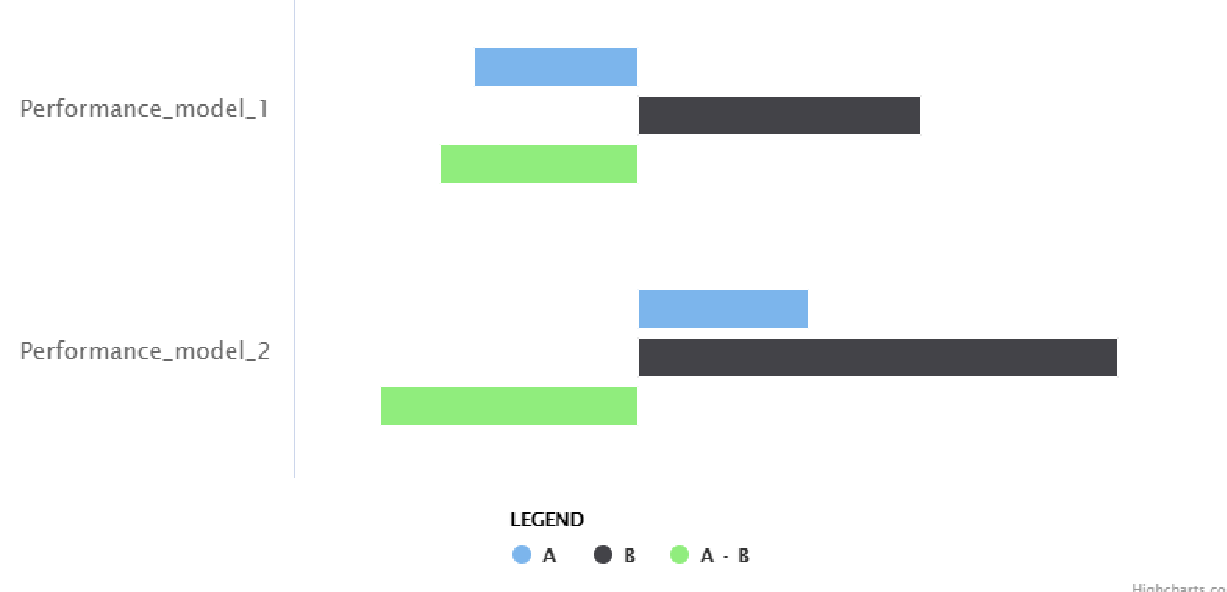
\includegraphics[width=15cm,height=15cm,keepaspectratio,]{pics/ratio_plot_with_positive_negative.pdf}
\caption[mockup1]{Mockup of ratio plot with configuration options A and B and interaction A $\cdot$ B for two performance-influence models, with separation between negative influences to the left side and positive influences to the right side of the center axis}
\end{figure}

Another improvement on ratio plot would be to show all the configuration options and interactions in the same order for all the performance-influence models. Currently, we display the configuration options and interactions in a sorted order from highest to lowest performance influence for each performance-influence model, which makes comparison a difficult task.  \hyperref[sameOrder]{Figure 7.2}, is a mock-up of the same.

\begin{figure}[ht]
\centering
\label{sameOrder}
 %- \textbf{Your title}\par\medskip
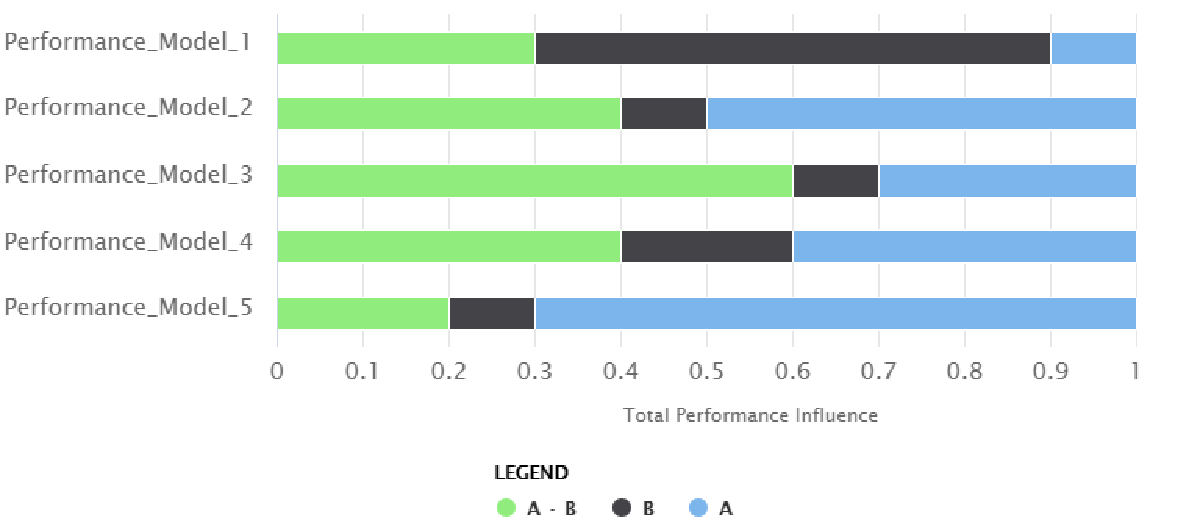
\includegraphics[width=15cm,height=15cm,keepaspectratio,]{pics/ratio_plot_without_sorted_order.pdf}
\caption[mockup2]{Mockup of ratio plot with configuration options A and B and interaction A $\cdot$ B of 5 performance-influence models all displayed in the same order}
\end{figure}


An improvement suggested for radar and text plot was to present the configuration options and interactions in a sorted order. This would help the users perception in finding the most relevant configuration option or interaction easily.



%*********************************************************************%
% APPENDIX                                                             %
%*********************************************************************%

\appendix
\ifgerman{\chapter{Anhang}}{\chapter{Appendix}}
\label{appedixa}

\section{Difficulty Rating vs Time measurements co-relation}
\label{sanityCheck}
Sanity check is made to ensure that the assumption made from the results of difficulty rating hold true. To conduct the sanity check, we plot graphs with difficulty rating against time taken to answer a question, per interviewee.

\begin{figure}[H]
\centering
\begin{adjustbox}{width=1\textwidth}
\begin{minipage}[8cm]{.44\textwidth}
\begin{tikzpicture}[scale=0.80]
	\begin{axis}[%
	xlabel={Difficulty Ratings},
    ylabel={Time(in seconds)},
    ymin=0,
    minor y tick num=2,
    grid style={dashed,gray!30},
    ymajorgrids=true,
    xmajorgrids=true,
    yminorgrids=true,
    only marks,
    scatter,
    mark size=3.5pt,
    scatter src=explicit symbolic,
	scatter/classes={
		a={mark=square,draw=gray},
		b={mark=triangle,draw=gray},
		c={mark=otimes,draw=gray},
		x={mark=diamond,draw=gray},
	    y={mark=oplus,draw=gray},
		z={mark=star,draw=gray},
		q1sRa={mark=square,draw=green},
	    q1sT={mark=triangle,draw=green},
		q1sRo={mark=otimes,draw=green},
		q1cRa={mark=diamond,draw=green},
	    q1cT={mark=oplus,draw=green},
		q1cRo={mark=star,draw=green},
		q2sRa={mark=square,draw=orange},
	    q2sT={mark=triangle,draw=orange},
		q2sRo={mark=otimes,draw=orange},
		q2cRa={mark=diamond,draw=orange},
	    q2cT={mark=oplus,draw=orange},
		q2cRo={mark=star,draw=orange},
		q3sRa={mark=square,draw=blue},
	    q3sT={mark=triangle,draw=blue},
		q3sRo={mark=otimes,draw=blue},
		q3cRa={mark=diamond,draw=blue},
	    q3cT={mark=oplus,draw=blue},
		q3cRo={mark=star,draw=blue},
		q4sRa={mark=square,draw=red},
	    q4sT={mark=triangle,draw=red},
		q4sRo={mark=otimes,draw=red},
		q4cRa={mark=diamond,draw=red},
	    q4cT={mark=oplus,draw=red},
		q4cRo={mark=star,draw=red},
		q5sRa={mark=square,draw=black},
	    q5sT={mark=triangle,draw=black},
		q5sRo={mark=otimes,draw=black},
		q5cRa={mark=diamond,draw=black},
	    q5cT={mark=oplus,draw=black},
		q5cRo={mark=star,draw=black},
		q6sRa={mark=square,draw=cyan},
	    q6sT={mark=triangle,draw=cyan},
		q6sRo={mark=otimes,draw=cyan},
		q6cRa={mark=diamond,draw=cyan},
	    q6cT={mark=oplus,draw=cyan},
		q6cRo={mark=star,draw=cyan}},]
	\addplot[scatter,only marks,%
		scatter src=explicit symbolic]%
	table[meta=label] {
x         y         label
2	11.21	q1sRa
2	10.679	q1sT
1	13.292	q1sRo
		
3	30.59	q1cRa
3	25.252	q1cT
1	26.866	q1cRo
		
		
2	44.209	q2sRa
1	27.535	q2sT
5	70.4	q2sRo
		
3	39.415	q2cRa
3	32.897	q2cT
		
		
2	13.983	q3sRa
2	15.166	q3sT
5	34.07	q3sRo
		
4	53.26	q3cRa
2	23.036	q3cT
3	61.0	q3cRo
		
		
19

1	12.843	q4sRa
2	15.801	q4sT
4	32.092	q4sRo
		
2	28.282	q4cRa
2	30.629	q4cT
3	334.0	q4cRo
		
		
5	70.056	q5sRa
2	132.19	q5sT
4   110	    q5sRo
		
3	24.874	q5cRa
2	41.139	q5cT
4	68.315	q5cRo
		
		
2	102.026	q6sRa
4	32.672	q6sT
3	47.104	q6sRo
		
2	20.264	q6cRa
2	54.906	q6cT
5	55.942	q6cRo
};
\end{axis}
\begin{axis}[
    xmin=0,
    xmax=100,
    ymin=1,
    ymax=6,
    hide axis,
    only marks,
    ]
\foreach \i in {0,...,6} {
        \addplot+ [mark=*] coordinates { (0,0) };
     }
    \end{axis}
\end{tikzpicture}
\caption{Difficulty rating and time measurements for interviewee 1}\label{figure:interviewee1}
\vspace{\baselineskip}
\end{minipage}
\begin{minipage}[8cm]{.44\textwidth}
\begin{tikzpicture}[scale=0.80]
	\begin{axis}[%
	xlabel={Difficulty Ratings},
    ylabel={Time(in seconds)},
    ymin=0,
    minor y tick num=2,
    grid style={dashed,gray!30},
    ymajorgrids=true,
    xmajorgrids=true,
    yminorgrids=true,
    only marks,
    scatter,
    mark size=3.5pt,
    scatter src=explicit symbolic,
	scatter/classes={
		a={mark=square,draw=gray},
		b={mark=triangle,draw=gray},
		c={mark=otimes,draw=gray},
		x={mark=diamond,draw=gray},
	    y={mark=oplus,draw=gray},
		z={mark=star,draw=gray},
		q1sRa={mark=square,draw=green},
	    q1sT={mark=triangle,draw=green},
		q1sRo={mark=otimes,draw=green},
		q1cRa={mark=diamond,draw=green},
	    q1cT={mark=oplus,draw=green},
		q1cRo={mark=star,draw=green},
		q2sRa={mark=square,draw=orange},
	    q2sT={mark=triangle,draw=orange},
		q2sRo={mark=otimes,draw=orange},
		q2cRa={mark=diamond,draw=orange},
	    q2cT={mark=oplus,draw=orange},
		q2cRo={mark=star,draw=orange},
		q3sRa={mark=square,draw=blue},
	    q3sT={mark=triangle,draw=blue},
		q3sRo={mark=otimes,draw=blue},
		q3cRa={mark=diamond,draw=blue},
	    q3cT={mark=oplus,draw=blue},
		q3cRo={mark=star,draw=blue},
		q4sRa={mark=square,draw=red},
	    q4sT={mark=triangle,draw=red},
		q4sRo={mark=otimes,draw=red},
		q4cRa={mark=diamond,draw=red},
	    q4cT={mark=oplus,draw=red},
		q4cRo={mark=star,draw=red},
		q5sRa={mark=square,draw=black},
	    q5sT={mark=triangle,draw=black},
		q5sRo={mark=otimes,draw=black},
		q5cRa={mark=diamond,draw=black},
	    q5cT={mark=oplus,draw=black},
		q5cRo={mark=star,draw=black},
		q6sRa={mark=square,draw=cyan},
	    q6sT={mark=triangle,draw=cyan},
		q6sRo={mark=otimes,draw=cyan},
		q6cRa={mark=diamond,draw=cyan},
	    q6cT={mark=oplus,draw=cyan},
		q6cRo={mark=star,draw=cyan}}]
	\addplot[scatter,only marks,%
		scatter src=explicit symbolic]%
	table[meta=label] {
x         y         label
		
		
1	10.2	q1sRa
1	3.23	q1sT
1	10.45	q1sRo
		
2	10.12	q1cRa
2	7.02	q1cT
2	14.33	q1cRo
		
		
2	22.27	q2sRa
3	16.11	q2sT
3	30.6	q2sRo
		
2	32.19	q2cRa
2	21.49	q2cT
		
		
2	21.64	q3sRa
2	6	q3sT
2	20.43	q3sRo
		
2	19.82	q3cRa
2	14.88	q3cT
2	21.84	q3cRo
		
		
2	9.07	q4sRa
2	7.04	q4sT
3	24.2	q4sRo
		
3	21.71	q4cRa
2	15.53	q4cT
4	35.03	q4cRo
		
		
3	43.14	q5sRa
2	25.58	q5sT
5	73.39	q5sRo
		
4	52.97	q5cRa
1	24.97	q5cT
5	6.33	q5cRo
		
		
4	41.64	q6sRa
4	65.88	q6sT
5	11.25	q6sRo
		
2	29.91	q6cRa
2	19.16	q6cT
5	14.82	q6cRo

};
\end{axis}
	
\begin{axis}[
    xmin=0,
    xmax=100,
    ymin=1,
    ymax=6,
    hide axis,
    only marks,
    ]
\foreach \i in {0,...,6} {
        \addplot+ [mark=*] coordinates { (0,0) };
     }
    \end{axis}
\end{tikzpicture}
\caption{Difficulty rating and time measurements for interviewee 2} 
\label{figure:interviewee2}
\vspace{\baselineskip}
\end{minipage}



\end{adjustbox}
\end{figure}

\begin{figure}[H]
\centering
\begin{adjustbox}{width=1\textwidth}
\begin{minipage}[8cm]{.44\textwidth}
\begin{tikzpicture}[scale=0.80]
	\begin{axis}[%
	xlabel={Difficulty Ratings},
    ylabel={Time(in seconds)},
    ymin=0,
    minor y tick num=2,
    grid style={dashed,gray!30},
    ymajorgrids=true,
    xmajorgrids=true,
    yminorgrids=true,
    only marks,
    scatter,
    mark size=3.5pt,
    scatter src=explicit symbolic,
	scatter/classes={
		a={mark=square,draw=gray},
		b={mark=triangle,draw=gray},
		c={mark=otimes,draw=gray},
		x={mark=diamond,draw=gray},
	    y={mark=oplus,draw=gray},
		z={mark=star,draw=gray},
		q1sRa={mark=square,draw=green},
	    q1sT={mark=triangle,draw=green},
		q1sRo={mark=otimes,draw=green},
		q1cRa={mark=diamond,draw=green},
	    q1cT={mark=oplus,draw=green},
		q1cRo={mark=star,draw=green},
		q2sRa={mark=square,draw=orange},
	    q2sT={mark=triangle,draw=orange},
		q2sRo={mark=otimes,draw=orange},
		q2cRa={mark=diamond,draw=orange},
	    q2cT={mark=oplus,draw=orange},
		q2cRo={mark=star,draw=orange},
		q3sRa={mark=square,draw=blue},
	    q3sT={mark=triangle,draw=blue},
		q3sRo={mark=otimes,draw=blue},
		q3cRa={mark=diamond,draw=blue},
	    q3cT={mark=oplus,draw=blue},
		q3cRo={mark=star,draw=blue},
		q4sRa={mark=square,draw=red},
	    q4sT={mark=triangle,draw=red},
		q4sRo={mark=otimes,draw=red},
		q4cRa={mark=diamond,draw=red},
	    q4cT={mark=oplus,draw=red},
		q4cRo={mark=star,draw=red},
		q5sRa={mark=square,draw=black},
	    q5sT={mark=triangle,draw=black},
		q5sRo={mark=otimes,draw=black},
		q5cRa={mark=diamond,draw=black},
	    q5cT={mark=oplus,draw=black},
		q5cRo={mark=star,draw=black},
		q6sRa={mark=square,draw=cyan},
	    q6sT={mark=triangle,draw=cyan},
		q6sRo={mark=otimes,draw=cyan},
		q6cRa={mark=diamond,draw=cyan},
	    q6cT={mark=oplus,draw=cyan},
		q6cRo={mark=star,draw=cyan}},]
	\addplot[scatter,only marks,%
		scatter src=explicit symbolic]%
	table[meta=label] {
x         y         label
2	5.024	q1sRa
2	10.598	q1sT
1	8.192	q1sRo
		
3	17.776	q1cRa
2	24.036	q1cT
1	13.924	q1cRo
		
		
3	28.976	q2sRa
3	22.55	q2sT
4	71.008	q2sRo
		
2	30.775	q2cRa
2	28.218	q2cT
		
		
2	21.04	q3sRa
2	26.556	q3sT
5	144.0	q3sRo
		
3	69.0	q3cRa
2	28.73	q3cT
3	35.122	q3cRo
		
		
2	28.97	q4sRa
2	31.51	q4sT
5	139.0	q4sRo
		
3	26.741	q4cRa
2	28.969	q4cT
3	72.741	q4cRo
		
		
3	85.5	q5sRa
4	99.7	q5sT
5	313.555	q5sRo
		
4	171.4	q5cRa
3	196.8	q5cT
5	146.903	q5cRo
		
		
3	49.043	q6sRa
3	110.686	q6sT
5	159.1	q6sRo
		
3	51.01	q6cRa
3	40.757	q6cT
5	288.940	q6cRo
};
\end{axis}
	
\begin{axis}[
    xmin=0,
    xmax=100,
    ymin=1,
    ymax=6,
    hide axis,
    only marks,
    ]
\foreach \i in {0,...,6} {
        \addplot+ [mark=*] coordinates { (0,0) };
     }
    \end{axis}
\end{tikzpicture}
\caption{Difficulty rating and time measurements for interviewee 3}\label{figure:interviewee3}
\vspace{\baselineskip}
\end{minipage}
\begin{minipage}[8cm]{.44\textwidth}
\begin{tikzpicture}[scale=0.80]
	\begin{axis}[%
	xlabel={Difficulty Ratings},
    ylabel={Time(in seconds)},
    ymin=0,
    minor y tick num=2,
    grid style={dashed,gray!30},
    ymajorgrids=true,
    xmajorgrids=true,
    yminorgrids=true,
    only marks,
    scatter,
    mark size=3.5pt,
    scatter src=explicit symbolic,
	scatter/classes={
		a={mark=square,draw=gray},
		b={mark=triangle,draw=gray},
		c={mark=otimes,draw=gray},
		x={mark=diamond,draw=gray},
	    y={mark=oplus,draw=gray},
		z={mark=star,draw=gray},
		q1sRa={mark=square,draw=green},
	    q1sT={mark=triangle,draw=green},
		q1sRo={mark=otimes,draw=green},
		q1cRa={mark=diamond,draw=green},
	    q1cT={mark=oplus,draw=green},
		q1cRo={mark=star,draw=green},
		q2sRa={mark=square,draw=orange},
	    q2sT={mark=triangle,draw=orange},
		q2sRo={mark=otimes,draw=orange},
		q2cRa={mark=diamond,draw=orange},
	    q2cT={mark=oplus,draw=orange},
		q2cRo={mark=star,draw=orange},
		q3sRa={mark=square,draw=blue},
	    q3sT={mark=triangle,draw=blue},
		q3sRo={mark=otimes,draw=blue},
		q3cRa={mark=diamond,draw=blue},
	    q3cT={mark=oplus,draw=blue},
		q3cRo={mark=star,draw=blue},
		q4sRa={mark=square,draw=red},
	    q4sT={mark=triangle,draw=red},
		q4sRo={mark=otimes,draw=red},
		q4cRa={mark=diamond,draw=red},
	    q4cT={mark=oplus,draw=red},
		q4cRo={mark=star,draw=red},
		q5sRa={mark=square,draw=black},
	    q5sT={mark=triangle,draw=black},
		q5sRo={mark=otimes,draw=black},
		q5cRa={mark=diamond,draw=black},
	    q5cT={mark=oplus,draw=black},
		q5cRo={mark=star,draw=black},
		q6sRa={mark=square,draw=cyan},
	    q6sT={mark=triangle,draw=cyan},
		q6sRo={mark=otimes,draw=cyan},
		q6cRa={mark=diamond,draw=cyan},
	    q6cT={mark=oplus,draw=cyan},
		q6cRo={mark=star,draw=cyan}},]
	\addplot[scatter,only marks,%
		scatter src=explicit symbolic]%
	table[meta=label] {
x         y         label
		
		
1	20.089	q1sRa
1	24.125	q1sT
2	20.362	q1sRo
		
1	6.124	q1cRa
1	10.416	q1cT
1	31.608	q1cRo
		
		
1	14.328	q2sRa
1	30.085	q2sT
5	15.913	q2sRo
		
1	14.296	q2cRa
2	29.725	q2cT
		
		
1	2.357	q3sRa
1	12.884	q3sT
4	11.979	q3sRo
		
5	20.154	q3cRa
2	7.927	q3cT
5	21.694	q3cRo
		
		
2	24.296	q4sRa
2	45.527	q4sT
4	91.9	q4sRo
		
2	25.298	q4cRa
2	35.165	q4cT
3	46.726	q4cRo
		
		
3	125.0	q5sRa
2	36.758	q5sT
5	45.017	q5sRo
		
2	13.229	q5cRa
2	24.62	q5cT
5	27.879	q5cRo
		
		
3	45.44	q6sRa
3	53.34	q6sT
4	68.346	q6sRo
		
2	54.65	q6cRa
2	34.56	q6cT
4	65.34	q6cRo

};
\end{axis}
	
\begin{axis}[
    xmin=0,
    xmax=100,
    ymin=1,
    ymax=6,
    hide axis,
    only marks,]
\foreach \i in {0,...,6} {
        \addplot+ [mark=*] coordinates { (0,0) };
     }
    \end{axis}
\end{tikzpicture}
\caption{Difficulty rating and time measurements for interviewee 4}\label{figure:interviewee4}
\vspace{\baselineskip}
\end{minipage}
\end{adjustbox}
\end{figure}

\begin{figure}[H]
\centering
\begin{adjustbox}{width=1\textwidth}
\begin{minipage}[8cm]{.44\textwidth}
\begin{tikzpicture}[scale=0.80]
	\begin{axis}[%
	xlabel={Difficulty Ratings},
    ylabel={Time(in seconds)},
    ymin=0,
    minor y tick num=2,
    grid style={dashed,gray!30},
    ymajorgrids=true,
    xmajorgrids=true,
    yminorgrids=true,
    only marks,
    scatter,
    mark size=3.5pt,
    scatter src=explicit symbolic,
	scatter/classes={
		a={mark=square,draw=gray},
		b={mark=triangle,draw=gray},
		c={mark=otimes,draw=gray},
		x={mark=diamond,draw=gray},
	    y={mark=oplus,draw=gray},
		z={mark=star,draw=gray},
		q1sRa={mark=square,draw=green},
	    q1sT={mark=triangle,draw=green},
		q1sRo={mark=otimes,draw=green},
		q1cRa={mark=diamond,draw=green},
	    q1cT={mark=oplus,draw=green},
		q1cRo={mark=star,draw=green},
		q2sRa={mark=square,draw=orange},
	    q2sT={mark=triangle,draw=orange},
		q2sRo={mark=otimes,draw=orange},
		q2cRa={mark=diamond,draw=orange},
	    q2cT={mark=oplus,draw=orange},
		q2cRo={mark=star,draw=orange},
		q3sRa={mark=square,draw=blue},
	    q3sT={mark=triangle,draw=blue},
		q3sRo={mark=otimes,draw=blue},
		q3cRa={mark=diamond,draw=blue},
	    q3cT={mark=oplus,draw=blue},
		q3cRo={mark=star,draw=blue},
		q4sRa={mark=square,draw=red},
	    q4sT={mark=triangle,draw=red},
		q4sRo={mark=otimes,draw=red},
		q4cRa={mark=diamond,draw=red},
	    q4cT={mark=oplus,draw=red},
		q4cRo={mark=star,draw=red},
		q5sRa={mark=square,draw=black},
	    q5sT={mark=triangle,draw=black},
		q5sRo={mark=otimes,draw=black},
		q5cRa={mark=diamond,draw=black},
	    q5cT={mark=oplus,draw=black},
		q5cRo={mark=star,draw=black},
		q6sRa={mark=square,draw=cyan},
	    q6sT={mark=triangle,draw=cyan},
		q6sRo={mark=otimes,draw=cyan},
		q6cRa={mark=diamond,draw=cyan},
	    q6cT={mark=oplus,draw=cyan},
		q6cRo={mark=star,draw=cyan}},]
	\addplot[scatter,only marks,%
		scatter src=explicit symbolic]%
	table[meta=label] {
x         y         label
1	33.57	q1sRa
2	23.46	q1sT
1	11.93	q1sRo
		
3	10.01	q1cRa
3	17.28	q1cT
2	15.46	q1cRo
		
		
1	30.98	q2sRa
1	13.76	q2sT
5	24.32	q2sRo
		
2	34.1	q2cRa
2	24.4	q2cT
		
		
2	30.68	q3sRa
2	7.45	q3sT
3	25.5	q3sRo
		
3	37.88	q3cRa
2	22.25	q3cT
3	54.98	q3cRo
		
		
2	15.45	q4sRa
1	10.9	q4sT
4	35.67	q4sRo
		
3	23.11	q4cRa
2	18.29	q4cT
5	60.23	q4cRo
		
		
3	146.31	q5sRa
3	56.9	q5sT
5	66.84	q5sRo
		
3	122.44	q5cRa
2	58.59	q5cT
5	40.88	q5cRo
		
		
3	74.57	q6sRa
3	38.44	q6sT
3	43.02	q6sRo
		
3	57.25	q6cRa
2	26.93	q6cT
4	83.55	q6cRo


};
\end{axis}
	
\begin{axis}[
    xmin=0,
    xmax=100,
    ymin=1,
    ymax=6,
    hide axis,
    only marks,
    ]
\foreach \i in {0,...,6} {
        \addplot+ [mark=*] coordinates { (0,0) };
     }
    \end{axis}
\end{tikzpicture}
\caption{Difficulty rating and time measurements for interviewee 5}\label{figure:interviewee5}
\vspace{\baselineskip}
\end{minipage}
\begin{minipage}[8cm]{.44\textwidth}
\begin{tikzpicture}[scale=0.80]
	\begin{axis}[%
	xlabel={Difficulty Ratings},
    ylabel={Time(in seconds)},
    ymin=0,
    minor y tick num=2,
    grid style={dashed,gray!30},
    ymajorgrids=true,
    xmajorgrids=true,
    yminorgrids=true,
    only marks,
    scatter,
    mark size=3.5pt,
    scatter src=explicit symbolic,
	scatter/classes={
		a={mark=square,draw=gray},
		b={mark=triangle,draw=gray},
		c={mark=otimes,draw=gray},
		x={mark=diamond,draw=gray},
	    y={mark=oplus,draw=gray},
		z={mark=star,draw=gray},
		q1sRa={mark=square,draw=green},
	    q1sT={mark=triangle,draw=green},
		q1sRo={mark=otimes,draw=green},
		q1cRa={mark=diamond,draw=green},
	    q1cT={mark=oplus,draw=green},
		q1cRo={mark=star,draw=green},
		q2sRa={mark=square,draw=orange},
	    q2sT={mark=triangle,draw=orange},
		q2sRo={mark=otimes,draw=orange},
		q2cRa={mark=diamond,draw=orange},
	    q2cT={mark=oplus,draw=orange},
		q2cRo={mark=star,draw=orange},
		q3sRa={mark=square,draw=blue},
	    q3sT={mark=triangle,draw=blue},
		q3sRo={mark=otimes,draw=blue},
		q3cRa={mark=diamond,draw=blue},
	    q3cT={mark=oplus,draw=blue},
		q3cRo={mark=star,draw=blue},
		q4sRa={mark=square,draw=red},
	    q4sT={mark=triangle,draw=red},
		q4sRo={mark=otimes,draw=red},
		q4cRa={mark=diamond,draw=red},
	    q4cT={mark=oplus,draw=red},
		q4cRo={mark=star,draw=red},
		q5sRa={mark=square,draw=black},
	    q5sT={mark=triangle,draw=black},
		q5sRo={mark=otimes,draw=black},
		q5cRa={mark=diamond,draw=black},
	    q5cT={mark=oplus,draw=black},
		q5cRo={mark=star,draw=black},
		q6sRa={mark=square,draw=cyan},
	    q6sT={mark=triangle,draw=cyan},
		q6sRo={mark=otimes,draw=cyan},
		q6cRa={mark=diamond,draw=cyan},
	    q6cT={mark=oplus,draw=cyan},
		q6cRo={mark=star,draw=cyan}}]
	\addplot[scatter,only marks,%
		scatter src=explicit symbolic]%
	table[meta=label] {
x         y         label
2	36.969	q1sRa
2	22.17	q1sT
1	16.967	q1sRo
		
2	24.232	q1cRa
3	32.167	q1cT
1	33.992	q1cRo
		
		
2	34.977	q2sRa
2	25.743	q2sT
2	43.967	q2sRo
		
2	18.869	q2cRa
2	36.871	q2cT
		
		
2	20.768	q3sRa
1	12.771	q3sT
3	29.559	q3sRo
		
1	13.532	q3cRa
2	16.686	q3cT
4	44.234	q3cRo
		
		
2	22.515	q4sRa
2	13.725	q4sT
3	33.804	q4sRo
		
3	25.71	q4cRa
2	24.5	q4cT
3	25.446	q4cRo
		
		
2	 67.798	q5sRa
2	40.329	q5sT
4	 76.052	q5sRo
		
2	21.658	q5cRa
2	54.374	q5cT
4	46.601	q5cRo
		
3	33.894	q6sRa
3	59.25	q6sT
5	715.016	q6sRo
		
2	55.654	q6cRa
2	39.917	q6cT
5	52.343	q6cRo
};
\end{axis}
	
\begin{axis}[
    xmin=0,
    xmax=100,
    ymin=1,
    ymax=6,
    hide axis,
    only marks,
    ]
\foreach \i in {0,...,6} {
        \addplot+ [mark=*] coordinates { (0,0) };
     }
    \end{axis}
\end{tikzpicture}
\caption{Difficulty rating and time measurements for interviewee 6}\label{figure:interviewee6}
\vspace{\baselineskip}
\end{minipage}
\end{adjustbox}
\end{figure}

\begin{figure}[H]
\centering
\begin{adjustbox}{width=1\textwidth}
\begin{minipage}[8cm]{.44\textwidth}
\begin{tikzpicture}[scale=0.80]
	\begin{axis}[%
	xlabel={Difficulty Ratings},
    ylabel={Time(in seconds)},
    ymin=0,
    minor y tick num=2,
    grid style={dashed,gray!30},
    ymajorgrids=true,
    xmajorgrids=true,
    yminorgrids=true,
    only marks,
    scatter,
    mark size=3.5pt,
    scatter src=explicit symbolic,
	scatter/classes={
		a={mark=square,draw=gray},
		b={mark=triangle,draw=gray},
		c={mark=otimes,draw=gray},
		x={mark=diamond,draw=gray},
	    y={mark=oplus,draw=gray},
		z={mark=star,draw=gray},
		q1sRa={mark=square,draw=green},
	    q1sT={mark=triangle,draw=green},
		q1sRo={mark=otimes,draw=green},
		q1cRa={mark=diamond,draw=green},
	    q1cT={mark=oplus,draw=green},
		q1cRo={mark=star,draw=green},
		q2sRa={mark=square,draw=orange},
	    q2sT={mark=triangle,draw=orange},
		q2sRo={mark=otimes,draw=orange},
		q2cRa={mark=diamond,draw=orange},
	    q2cT={mark=oplus,draw=orange},
		q2cRo={mark=star,draw=orange},
		q3sRa={mark=square,draw=blue},
	    q3sT={mark=triangle,draw=blue},
		q3sRo={mark=otimes,draw=blue},
		q3cRa={mark=diamond,draw=blue},
	    q3cT={mark=oplus,draw=blue},
		q3cRo={mark=star,draw=blue},
		q4sRa={mark=square,draw=red},
	    q4sT={mark=triangle,draw=red},
		q4sRo={mark=otimes,draw=red},
		q4cRa={mark=diamond,draw=red},
	    q4cT={mark=oplus,draw=red},
		q4cRo={mark=star,draw=red},
		q5sRa={mark=square,draw=black},
	    q5sT={mark=triangle,draw=black},
		q5sRo={mark=otimes,draw=black},
		q5cRa={mark=diamond,draw=black},
	    q5cT={mark=oplus,draw=black},
		q5cRo={mark=star,draw=black},
		q6sRa={mark=square,draw=cyan},
	    q6sT={mark=triangle,draw=cyan},
		q6sRo={mark=otimes,draw=cyan},
		q6cRa={mark=diamond,draw=cyan},
	    q6cT={mark=oplus,draw=cyan},
		q6cRo={mark=star,draw=cyan}},]
	\addplot[scatter,only marks,%
		scatter src=explicit symbolic]%
	table[meta=label] {
x         y         label
1	23.266	q1sRa
1	12.262	q1sT
1	18.282	q1sRo
		
2	39.292	q1cRa
2	16.376	q1cT
1	26.229	q1cRo
		
		
1	25.712	q2sRa
1	14.18	q2sT
5	42.934	q2sRo
		
2	26.911	q2cRa
2	22.574	q2cT
		
		
1	10.217	q3sRa
1	9.968	q3sT
1	30.947	q3sRo
		
2	56.401	q3cRa
2	12.044	q3cT
2	39.93	q3cRo
		
		
1	7.731	q4sRa
2	22.087	q4sT
2	27.443	q4sRo
		
2	26.379	q4cRa
2	9.274	q4cT
2	63.0	q4cRo
		
		
1	56.019	q5sRa
1	25.968	q5sT
4	97.1	q5sRo
		
1	18.88	q5cRa
1	25.893	q5cT
3	69.359	q5cRo
		
		
2	17.963	q6sRa
2	41.166	q6sT
2	27.851	q6sRo
		
2	17.708	q6cRa
2	17.255	q6cT
3	5.981	q6cRo

};
\end{axis}
	
\begin{axis}[
    xmin=0,
    xmax=100,
    ymin=1,
    ymax=6,
    hide axis,
    only marks,
    ]
\foreach \i in {0,...,6} {
        \addplot+ [mark=*] coordinates { (0,0) };
     }
    \end{axis}
\end{tikzpicture}
\caption{Difficulty rating and time measurements for interviewee 7}\label{figure:interviewee7}
\vspace{\baselineskip}
\end{minipage}
\begin{minipage}[8cm]{.44\textwidth}
\begin{tikzpicture}[scale=0.80]
	\begin{axis}[%
	xlabel={Difficulty Ratings},
    ylabel={Time(in seconds)},
    ymin=0,
    minor y tick num=2,
    grid style={dashed,gray!30},
    ymajorgrids=true,
    xmajorgrids=true,
    yminorgrids=true,
    only marks,
    scatter,
    mark size=3.5pt,
    scatter src=explicit symbolic,
	scatter/classes={
		a={mark=square,draw=gray},
		b={mark=triangle,draw=gray},
		c={mark=otimes,draw=gray},
		x={mark=diamond,draw=gray},
	    y={mark=oplus,draw=gray},
		z={mark=star,draw=gray},
		q1sRa={mark=square,draw=green},
	    q1sT={mark=triangle,draw=green},
		q1sRo={mark=otimes,draw=green},
		q1cRa={mark=diamond,draw=green},
	    q1cT={mark=oplus,draw=green},
		q1cRo={mark=star,draw=green},
		q2sRa={mark=square,draw=orange},
	    q2sT={mark=triangle,draw=orange},
		q2sRo={mark=otimes,draw=orange},
		q2cRa={mark=diamond,draw=orange},
	    q2cT={mark=oplus,draw=orange},
		q2cRo={mark=star,draw=orange},
		q3sRa={mark=square,draw=blue},
	    q3sT={mark=triangle,draw=blue},
		q3sRo={mark=otimes,draw=blue},
		q3cRa={mark=diamond,draw=blue},
	    q3cT={mark=oplus,draw=blue},
		q3cRo={mark=star,draw=blue},
		q4sRa={mark=square,draw=red},
	    q4sT={mark=triangle,draw=red},
		q4sRo={mark=otimes,draw=red},
		q4cRa={mark=diamond,draw=red},
	    q4cT={mark=oplus,draw=red},
		q4cRo={mark=star,draw=red},
		q5sRa={mark=square,draw=black},
	    q5sT={mark=triangle,draw=black},
		q5sRo={mark=otimes,draw=black},
		q5cRa={mark=diamond,draw=black},
	    q5cT={mark=oplus,draw=black},
		q5cRo={mark=star,draw=black},
		q6sRa={mark=square,draw=cyan},
	    q6sT={mark=triangle,draw=cyan},
		q6sRo={mark=otimes,draw=cyan},
		q6cRa={mark=diamond,draw=cyan},
	    q6cT={mark=oplus,draw=cyan},
		q6cRo={mark=star,draw=cyan}},]
	\addplot[scatter,only marks,%
		scatter src=explicit symbolic]%
	table[meta=label] {
x         y         label
1	12.97	q1sRa
2	16.75	q1sT
2	19.96	q1sRo
		
4	72.52	q1cRa
2	33.27	q1cT
2	30.29	q1cRo
		
		
1	17.26	q2sRa
1	26.77	q2sT
5	45.15	q2sRo
		
2	27.76	q2cRa
2	11.9	q2cT
		
		
1	5.23	q3sRa
3	26	    q3sT
3	35.6	q3sRo
		
3	66.47	q3cRa
2	25.58	q3cT
4	92.75	q3cRo
		
		
2	12.42	q4sRa
2	18.63	q4sT
4	77.09	q4sRo
		
2	58.42	q4cRa
2	31.53	q4cT
4	27	    q4cRo
		
		
2	87.21	q5sRa
2	32.57	q5sT
2	22.02	q5sRo
		
3	31.42	q5cRa
2	26.34	q5cT
4	68.73	q5cRo
		
		
2	46.1	q6sRa
3	33.62	q6sT
3	12.92	q6sRo
		
3	25.29	q6cRa
5	33.85	q6cT
2	12.25	q6cRo
};
\end{axis}
	
\begin{axis}[
    xmin=0,
    xmax=100,
    ymin=1,
    ymax=6,
    hide axis,
    only marks,
    ]
\foreach \i in {0,...,6} {
        \addplot+ [mark=*] coordinates { (0,0) };
     }
    \end{axis}
\end{tikzpicture}
\caption{Difficulty rating and time measurements for interviewee 8}\label{figure:interviewee8}
\vspace{\baselineskip}
\end{minipage}
\end{adjustbox}
\end{figure}

\begin{figure}[ht]
\begin{tikzpicture}
	\begin{axis}[%
	xlabel={Difficulty Ratings},
    ylabel={Time(in seconds)},
    ymin=0,
    minor y tick num=2,
    grid style={dashed,gray!30},
    ymajorgrids=true,
    xmajorgrids=true,
    yminorgrids=true,
    only marks,
    scatter,
    mark size=3.5pt,
    scatter src=explicit symbolic,
	scatter/classes={
		a={mark=square,draw=gray},
		b={mark=triangle,draw=gray},
		c={mark=otimes,draw=gray},
		x={mark=diamond,draw=gray},
	    y={mark=oplus,draw=gray},
		z={mark=star,draw=gray},
		q1sRa={mark=square,draw=green},
	    q1sT={mark=triangle,draw=green},
		q1sRo={mark=otimes,draw=green},
		q1cRa={mark=diamond,draw=green},
	    q1cT={mark=oplus,draw=green},
		q1cRo={mark=star,draw=green},
		q2sRa={mark=square,draw=orange},
	    q2sT={mark=triangle,draw=orange},
		q2sRo={mark=otimes,draw=orange},
		q2cRa={mark=diamond,draw=orange},
	    q2cT={mark=oplus,draw=orange},
		q2cRo={mark=star,draw=orange},
		q3sRa={mark=square,draw=blue},
	    q3sT={mark=triangle,draw=blue},
		q3sRo={mark=otimes,draw=blue},
		q3cRa={mark=diamond,draw=blue},
	    q3cT={mark=oplus,draw=blue},
		q3cRo={mark=star,draw=blue},
		q4sRa={mark=square,draw=red},
	    q4sT={mark=triangle,draw=red},
		q4sRo={mark=otimes,draw=red},
		q4cRa={mark=diamond,draw=red},
	    q4cT={mark=oplus,draw=red},
		q4cRo={mark=star,draw=red},
		q5sRa={mark=square,draw=black},
	    q5sT={mark=triangle,draw=black},
		q5sRo={mark=otimes,draw=black},
		q5cRa={mark=diamond,draw=black},
	    q5cT={mark=oplus,draw=black},
		q5cRo={mark=star,draw=black},
		q6sRa={mark=square,draw=cyan},
	    q6sT={mark=triangle,draw=cyan},
		q6sRo={mark=otimes,draw=cyan},
		q6cRa={mark=diamond,draw=cyan},
	    q6cT={mark=oplus,draw=cyan},
		q6cRo={mark=star,draw=cyan}},
	     legend entries={
            Radar Plot-- Simple,
            Text Plot -- Simple,
            Ratio Plot -- Simple,
            Radar Plot-- Complex,
            Text Plot -- Complex,
            Ratio Plot -- Complex%
        },
        legend pos=outer north east,]
	\addplot[scatter,only marks,%
		scatter src=explicit symbolic]%
	table[meta=label] {
x         y         label
1	8.19	q1sRa
1	15.81	q1sT
1	13.01	q1sRo
		
2	26.52	q1cRa
2	30.77	q1cT
1	10.91	q1cRo
		
		
1	31.33	q2sRa
1	36.28	q2sT
4	31.37	q2sRo
		
1	24.92	q2cRa
1	13.77	q2cT
		
		
1	2.32	q3sRa
1	6.62	q3sT
2	26.28	q3sRo
		
3	37.64	q3cRa
3	30.79	q3cT
5	45.01	q3cRo
		
		
1	20.42	q4sRa
1	14.46	q4sT
5	48.84	q4sRo
		
2	14.34	q4cRa
1	14.04	q4cT
5	29.74	q4cRo
		
		
2	63.85	q5sRa
2	30.57	q5sT
5	131.0	q5sRo
		
4	74.6	q5cRa
1	21.09	q5cT
5	50.3	q5cRo
		
		
3	63.56	q6sRa
2	100.91	q6sT
3	37.49	q6sRo
		
2	31.43	q6cRa
3	65.0	q6cT
5	204.0	q6cRo

};
\end{axis}
	
\begin{axis}[
    xmin=0,
    xmax=100,
    ymin=1,
    ymax=6,
    hide axis,
    only marks,
    legend entries={
     ,   % the dummy plot should not show up in the legend
     Q1,Q2,Q3,Q4,Q5,Q6%
    },
    legend pos=outer north east,
    legend style={
            legend columns=-1, yshift=-100pt,
        },
    ]
\foreach \i in {0,...,6} {
        \addplot+ [mark=*] coordinates { (0,0) };
     }
    \end{axis}
\end{tikzpicture}
\label{figure:interviewee9}
\caption[Difficulty rating and time measurements for interviewee 9]{Difficulty rating and time measurements for interviewee 9} 
\end{figure}


\section{Questionnaire}
\label{appendix:questionnaire}
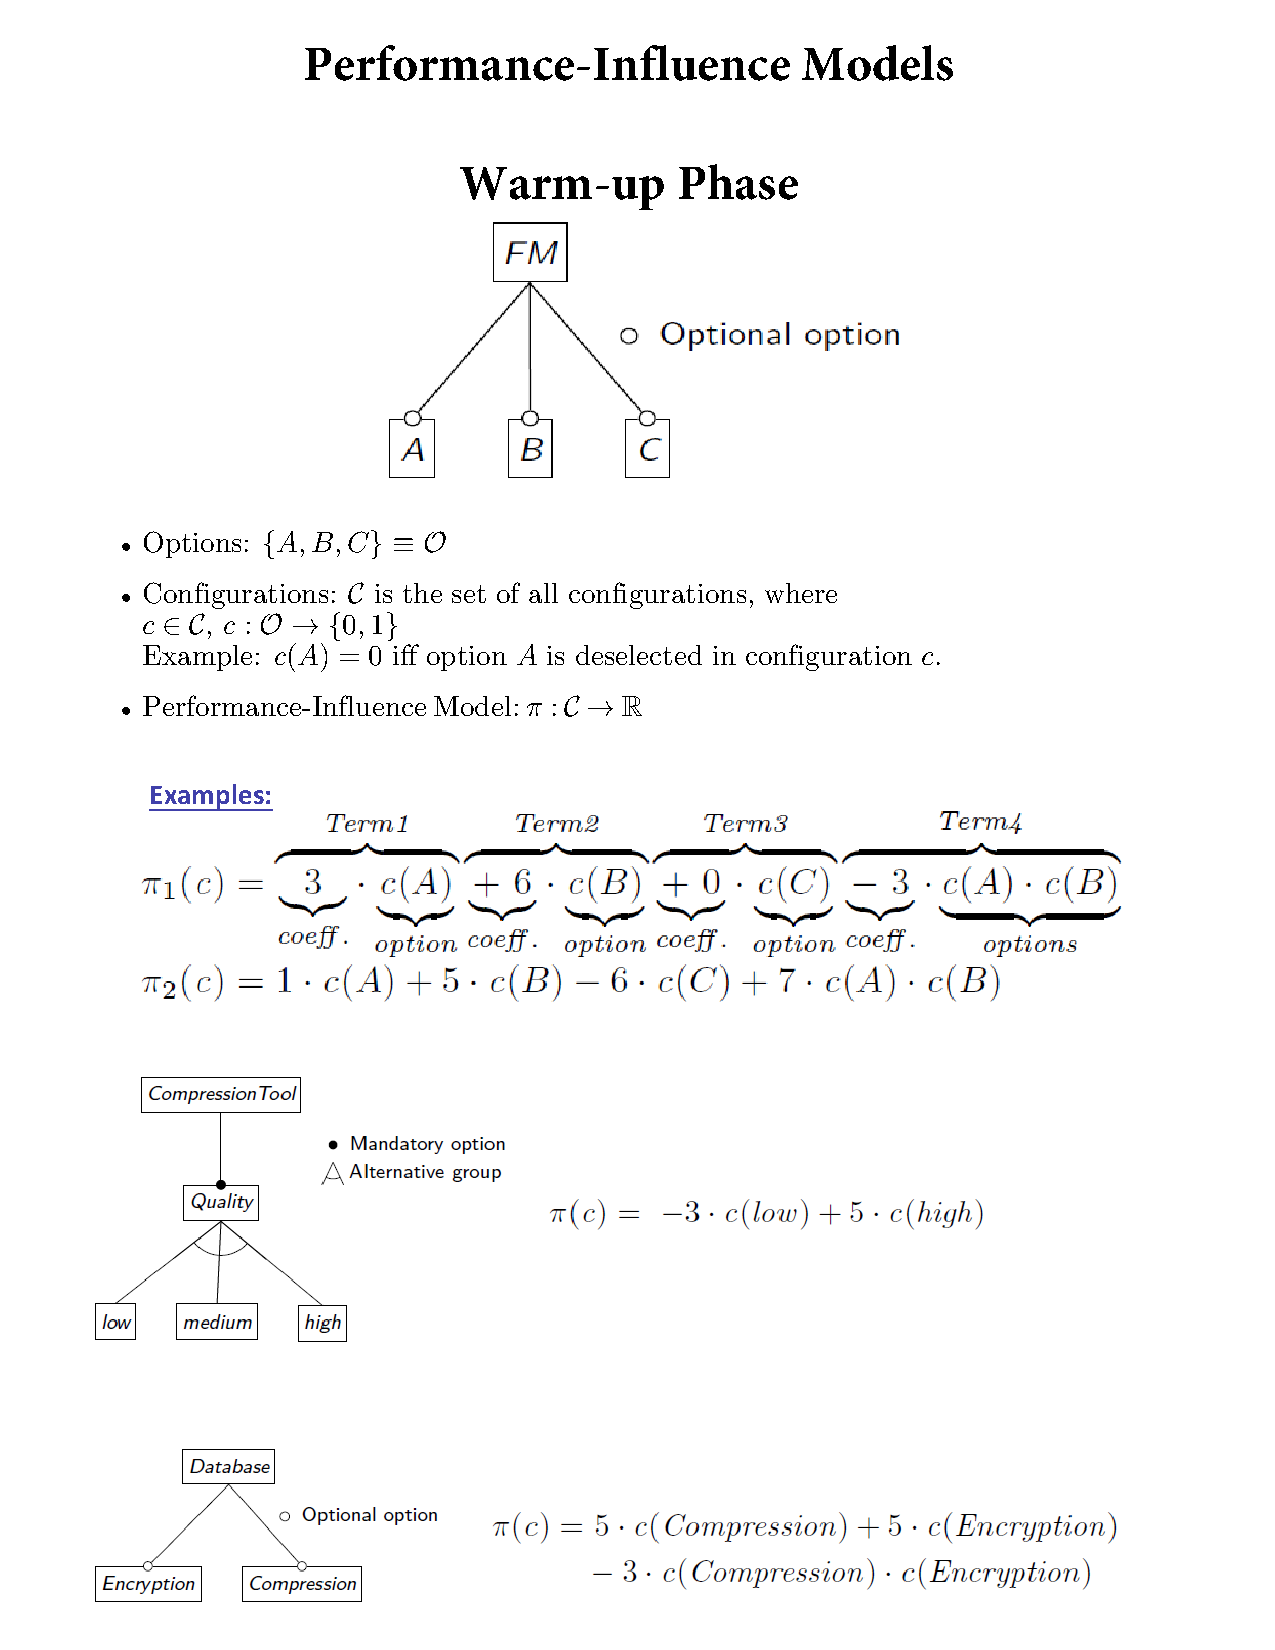
\includepdf[pages=-]{literature/Interview_Questionnaire.pdf}


%*********************************************************************%
% LITERATURE                                                          %
%*********************************************************************%

\cleardoublepage
\phantomsection 
\addcontentsline{toc}{chapter}{\bibname} % 
\bibliographystyle{alpha} % plain gerplain abbrvnat unsrtnat alphag alpha
% in a thesis you have space... use full names
\bibliography{literature/IEEEfull,literature/MYfull,literature/literature}
% in a paper, space is limited. use abreviations
%\bibliography{../literature/IEEEabrv,../literature/MYabrv,../literature/literature}

%*********************************************************************%
% ERKLÄRUNG                                                           %
%*********************************************************************%

\ifnotdraft{
	\cleardoublepage
	\phantomsection
	\printindex
	\thispagestyle{empty}
\vspace*{25\baselineskip}
\hbox to \textwidth{\hrulefill}
\par
\textbf{Eidesstattliche Erklärung:}

Hiermit versichere ich an Eides statt, dass ich diese Masterarbeit selbständig und
ohne Benutzung anderer als der angegebenen Quellen und Hilfsmittel angefertigt
habe und dass alle Ausführung\-en, die wörtlich oder sinngemäß übernommen wurden,
als solche gekenn\-zeichnet sind, sowie dass ich die Masterarbeit in gleicher oder
ähnlicher Form noch keiner anderen Prüfungsbehörde vorgelegt habe.

I hereby certify that this master’s thesis has been composed by myself, and describes my own work, unless otherwise acknowledged in the text. All references and verbatim extracts have been quoted, and all sources of information have been specifically acknowledged. It has not been submitted in any other application for a
degree.

\vspace*{20pt}

Rima Celita Lewis

Passau, den \thefullgermandate
%
% Hiermit erkl\"are ich, dass ich die vorliegende Arbeit selbst\"andig verfasst und
% keine anderen als die angegebenen Quellen und Hilfsmittel verwendet habe.
%
% Magdeburg, den \todots

%%%%%%%%%%%%%%%%%%%%%%%%%%%%%%%%%%%%%%%%%%%%%%%%%%%%%%%%%%%%%%%%%%%%%%%%
%% Hinweis:
%%
%% Diese Erklärung wird von der Prüfungsordnung für Diplomarbeiten
%% verlangt und ist zu unterschreiben. Für Studienarbeiten ist diese
%% Erklärung nicht zwingend notwendig, schadet aber auch nicht.
%%%%%%%%%%%%%%%%%%%%%%%%%%%%%%%%%%%%%%%%%%%%%%%%%%%%%%%%%%%%%%%%%%%%%%%%
\clearpage

}

\end{document}
